\documentclass[a4paper, twocolumn]{jarticle}
%\documentclass[uplatex]{jsarticle}
\usepackage[dvipdfmx]{graphicx}
\usepackage{float}
%\usepackage[dvips]{color}
%\usepackage{ascmac}
%\usepackage{verbatim}
\usepackage{setspace}
\usepackage[top=20mm,bottom=20mm,left=18mm,right=18mm]{geometry}
\makeatletter
\def\section{\@startsection{section}{1}{\z@}%
 {.1\Cvs \@plus.1\Cdp \@minus.1\Cdp}%
 {.1\Cvs \@plus.1\Cdp}%
 {\normalfont\normalsize\bfseries}}
\renewcommand{\thesection}{\arabic{section}.}
\renewcommand{\thesubsection}{\arabic{section}.\arabic{subsection}}
\def\subsection{\@startsection{subsection}{1}{\z@}%
 {.1\Cvs \@plus.1\Cdp \@minus.1\Cdp}%
 {.1\Cvs \@plus.1\Cdp}%
 {\normalfont\normalsize\bfseries}}

\def\@maketitle {
	\begin{center}
		\fontsize{14pt}{0pt}\selectfont
                % {\bf \@title{}}
                {\@title{}}
	\end{center}
	\vspace{1pt}
	\begin{flushleft}
		% \@author{指導教員 福田浩章 }
		\hfill{MA17099 古橋健斗}
	\end{flushleft}
\vspace{0.3cm}
}

%\makeatother
%\makeatletter

\renewcommand{\baselinestretch}{0.80}

\pagestyle{empty}
\makeatother

\begin{document}
\title{Kawaiiを探して\\KAWAII Quest -ルンバの大冒険-}
\date{}
\maketitle
\thispagestyle{empty}

\maketitle
%%%%%%%%%%%%%%%%%%%%%%%%%%%%%%%%%%%%%%%%
%%背景と目的
%%%%%%%%%%%%%%%%%%%%%%%%%%%%%%%%%%%%%%%%
% \section{研究の背景と目的}
% 阪神・淡路大震災をきっかけに,ロボット機器による災害救助ロボットの研究が
% 活発に行われるようになり,レスキューロボットの開発が本格化した.
% この問題に関しては,災害発生時には倒壊家具や瓦礫により被災者の発見が困難になり,
% また都市部被災では燃料などの可燃物の漏出や漏電などにより火災などの二次災害が発生し,
% 救援活動を行なう側が被災者となる危険性を含んでいる.
% 被災者の発見は災害救助犬などが存在するが,これには育成に時間とコストがかかり,勘と経験といった要素が含まれるため,一般的な問題となっている.
% そこで,これらを機械化することで災害による被害者を減らそうと言う思想が
% レスキューロボットの開発に繋がっている.
% ロボット技術を瓦礫の除去などに使用する試みがあったが,救助活動を行う人間の救助チーム
% だけではカバーすることができない.
% したがって,人間探索を行うロボット技術の開発に関する研究開発が進められている.
% また,福島第一原発事故の県から,危険箇所での作業者の被曝リスクを減らすために原子力
% 災害ロボットの導入や運用の重要性が再認識された.
% そのため,近年はロボット技術による探索技術が発展している.
%
% 一方,ディープラーニングは近年飛躍的な成長を遂げてきている.
% ディープラーニングとは,多層構造のニューラルネットワークを用いた機械学習である.
% 画像などのデータを入力し,情報がより深くの層に伝達している間に各層で学習を繰り返す.
% この過程で,使用者が設定した特徴量が自動で計算される.
% 特徴量とは,特定の概念を特徴づける変数のことである.
% この特徴量を発見できれば,パターン認識精度の向上や,問題の解決により近く.
% この階層的な特徴量の学習が,ディープラーニングが従来の機械学習と決定的に異なる.
% 判別機の学習には,正解画像が与えられれば1を,不正解画像が与えられれば
% 0を出力するように学習する.
% 大量のデータを判別機の学習に与えることで,より正確な判定ができるようになる.
%
% \section{提案}
% これらをふまえて,我々はディープラーニングを用いて対象物を判別し,効率的な情報収集を行うことができるロボットシステムの提案をする.
% 日本の誇れる文化であるゲーム・漫画やアニメーションなどのデジタルコンテンツが
% 大きな輸出超過になっている\cite{kawaii1}.
% その主要な要因として,高度な技術力とキャラクタのかわいさが挙げられることから,
% かわいいを人工物の感性価値として選び,かわいい人工物を対象として選択することにした.
% しかし,本研究はかわいい人工物を対象物とするが,ディープラーニングの教師データを変えることで,
% 様々な対象にも応用できるようロボットシステムの構築も目的とする.

\section{研究の背景と目的}

阪神・淡路大震災をきっかけに,ロボット機器による災害救助ロボットの研究が活発に行われるようになり,レスキューロボットの開発が本格化した.
この問題に関しては,災害発生時には倒壊家具や瓦礫により被災者の発見が困難になり,また都市部火災では燃料などの可燃物の漏出や漏電などにより火災などの二次災害が発生し,救援活動を行う側が被災者となる危険性を含んでいる.
被災者の発見は災害救助犬などが存在するが,これには育成に時間とコストがかかり,勘と経験といった要素が含まれるため,一般的な問題となっている.
そこで,これらを機械化することで,災害による被害者を減らそうという思想がレスキューロボットの開発に繋がっている.
人間の救助チームだけでは,災害現場の情報収集や人命救助に限界があるため,人間探索を行うロボット技術の開発が現在進められている.
また,福島第一原発事故の一件から,危険個所での作業者の被爆リスクを減らすために,原子力災害ロボットの導入や運用の重要性が再認識された.
そのため,近年はロボット技術による探索技術が発展している.

一方,ディープラーニングは近年飛躍的な成長を遂げてきている.
ディープラーニングとは,多層構造のニューラルネットワークを用いた機械学習である.
画像などのデータを入力し,情報がより深くの層に伝達している間に各層で学習を繰り返す.
この過程で,使用者が設定した特徴量が自動で計算される.
この特徴量は,物体認識をする際に用いられることがわかっている.
特定の物体認識の古典的手法として,物体の形状認識とパターンマッチングがある.
そこで我々は,ロボットの探索技術にディープラーニングを応用することで,効率的な情報収集を行うことが出来るロボットシステムを構築できるのではないかと考えた.

21世紀の社会において望まれるのは,物質的な豊かさでなく精神的な豊かさである.
さらに日本のものつくり産業に横たわる閉塞感を打破するために,従来のものつくりの価値観である性能・信頼性・価格に加え,感性を第4の価値として認識しようという国の取り組みも開始された.

研究代表者は,これまで行ってきた研究の成果を礎として,人工物(ものつくりの成果物)の感性価値の系統的な更生法の導出を目的とする研究を開始した.
「かわいい」を取り上げた理由は,日本のゲーム・漫画やアニメーションなどのデジタルコンテンツが世界中に広がっている要因として,日本人の高度できめ細やかな技術力と共に,キャラクタに「かわいい」という魅力があると考えられるからである.
そこで人工物の付加価値として「かわいい」という感性価値に注目し,その物理的属性を系統的に解析する研究を行ってきた\cite{thesis2}\cite{thesis3}.
これらをふまえて,我々はロボットに探索技術とディープラーニングを応用することで,ロボットに「かわいい」人工物を探索してもらい,「かわいい」の系統的解析をするための情報収集を行うことが出来るロボットシステムの構築と提案を目的とする.

本システムではロボットとしてルンバ\cite{roomba}を採用する.
ルンバは,iRobotが製造・販売するロボット掃除機であり,
部屋の中を単純なアルゴリズムに従って移動し,掃除を行う.
本システムでは,ルンバを掃除としてではなく,探索するロボットとして使用する.
そこで,本システムをKAWAII QUEST\~ルンバの大冒険\~と称し,以下にシステムの概要を述べる.

% システムの概要を説明.
\subsection{システムの概要}
\label{subsec:abstract}
本システムではルンバに学習モードと探索モードの2つのモードを搭載する.
\begin{enumerate}
  \item 学習モード\\ディープラーニングには大量の教師データ(画像データ)が必要となる.
  教師データを多く準備することが精度の向上に直接繋がる.
  また,個人によってかわいいと感じるものが異なる.
  そこで,本システム利用者がルンバを操作し,ルンバに搭載しているカメラを用いて教師データを
  収集する.
  これにより後述する探索モードで,本システム利用者毎に異なる分類器を作成することが可能になる.
  \item 探索モード\\本モードでは,ルンバが掃除を行うときに使用する単純な動作で部屋を徘徊する.
  そのときに,カメラに映った画像を解析し,物体を検知したときに作成した分類器で画像にかわいいものが
  映っているかを判別する.
  かわいいものが映っていれば,それを本システム利用者に表示し,かわいいかどうかを選択してもらう.
  かわいいと選択されるとその画像が保存され,正解教師データとして分類器を調節し,
  かわいくないと選択されると,その画像を不正解教師データとして分類器を調節する.
\end{enumerate}
以上の2つのモードを繰り返し使用することで,ユーザにあった判別器が作成され,判別の精度が向上する.
また,このモードを実現するために,以下の機器を使用する.

\begin{enumerate}
  \item ルンバ\\本システムの要である探索を行う.
  ルンバは,地図を作成せずに「らせん状に掃除する」「壁伝いに掃除する」
  「何かにぶつかったら角度を変えてランダムウォークする」などの単純なアルゴリズムで移動する.
  また,地図を作成することで同じ場所を探索しなくなり,より効率的な探索が可能になる.
  \item Kinect\\Kinect\cite{kinect}はマイクロソフトが発売したジェスチャー・音声認識によって操作ができるデバイスである.
  本システムではKinectをルンバに接続し,ルンバと連動して画像を撮影するために使用する.
  KinectとRobot Operating System(ROS)\cite{ros}を連動させることで,Kinectに映っている画像から物体検知を行うことが可能になる.
  \item ノートPC(ルンバに搭載)\\このPCでROSを動作させ,ルンバとKinectの連動を行う.
  他にも,撮影した画像をサーバに転送を行う.
  \item ノートPC(本システム利用者)\\このPCを使用し,対象物の選択や画像の閲覧を行う.
  また,学習モードではルンバの操作や画像の撮影が行える.
  これらを管理ツールと称し,ブラウザで管理できるような環境を構築する.
  \item RaspberryPi\\分類器の作成で画像処理を行うためには,高性能のPCが必要であるが,そのようなPCを用意するのは非常にコストがかかってしまう.
  そこで,本システムでは安価であるRaspberryPi\cite{rpi}を大量に使用し,効率よく画像処理を行える環境を構築する.
\end{enumerate}

\begin{table}[t]
	\centering
	\caption{RaspberryPi2 ModelBの性能}
	\label{tab:rpi2}
	{
		\small
		\begin{tabular}{|c|c|} \hline
		CPU & ARM Cortex-A7 クアッドコア 900MHz\\ \hline
		メモリ & 1GB\\ \hline
		ネットワーク & 10/100Mbpsイーサネット\\ \hline
		電源 & 900mA(4.5 \textasciitilde 5.5W)\\ \hline
		\end{tabular}
	}
\end{table}

次に,前述した画像処理を行うための大量のRaspberryPiを使用した環境について述べる.
本システムでは,表\ref{tab:rpi2}に示すRaspberryPI2 ModelBを利用し,Linux系専用OSであるRaspbian Jessie Lite\cite{raspbian}を実行する.
表\ref{tab:rpi2}の通り,通常のPCに比べて性能は劣るが,一台約5000円と安価であるため少ない費用で多くの数用意することができる.
この環境で分散的に処理が行うことで,低コストで高性能なクラスターを作成することができる.
RaspberryPiを用いたデータセンタの研究\cite{thesis1}がすでに行われているため,その有意性は存在する.
この環境をRaspberryPiCluster(RPC)と称し,詳細を後述する.

\begin{figure}[t]
	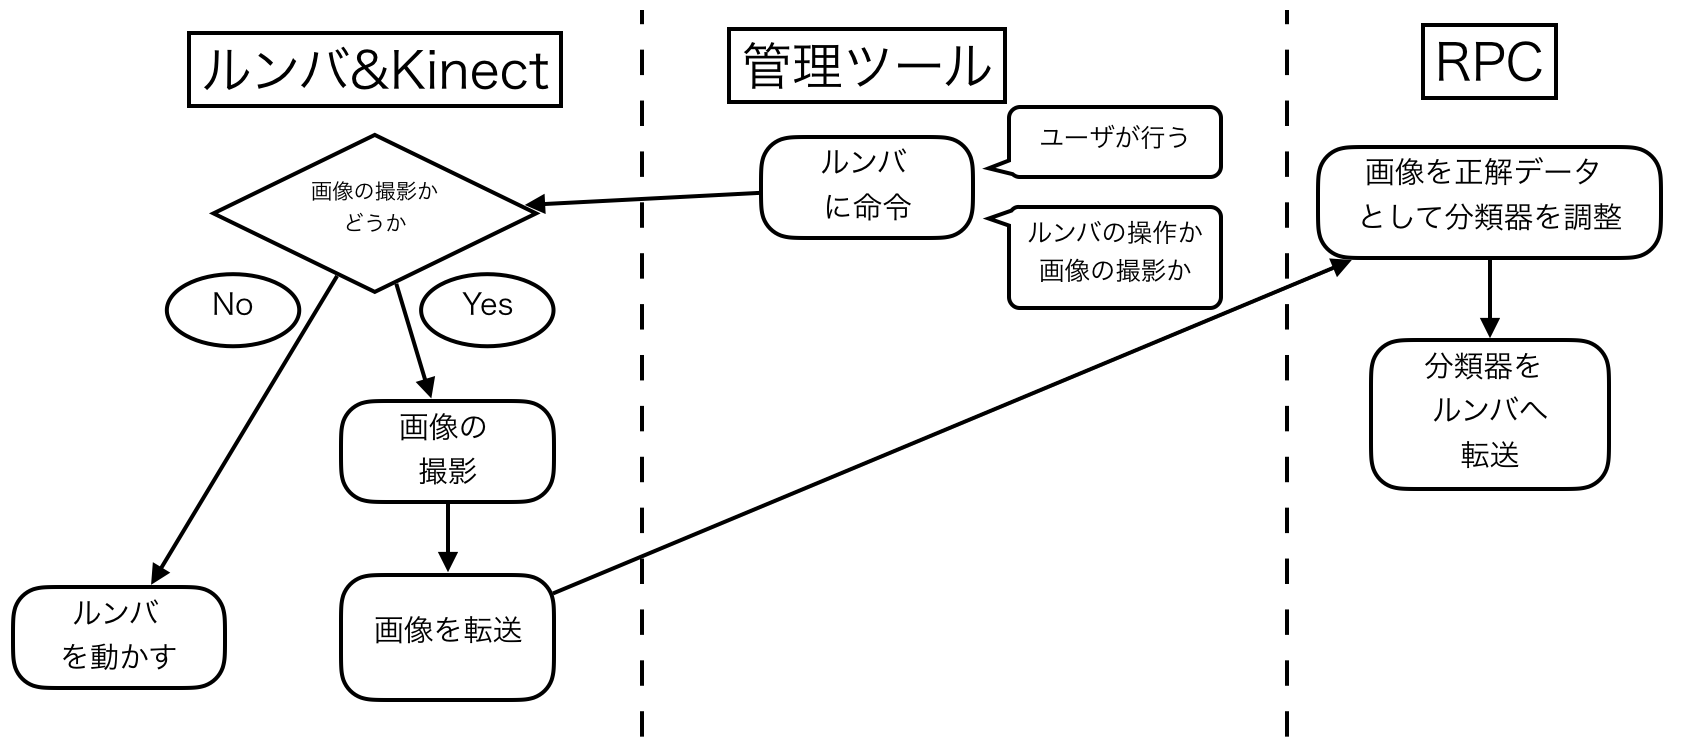
\includegraphics[width=8.5cm]{fig/flow_study.png}
	\caption{学習モードのフロー}
	\label{fig:learn_flow}
\end{figure}

\begin{figure}[t]
	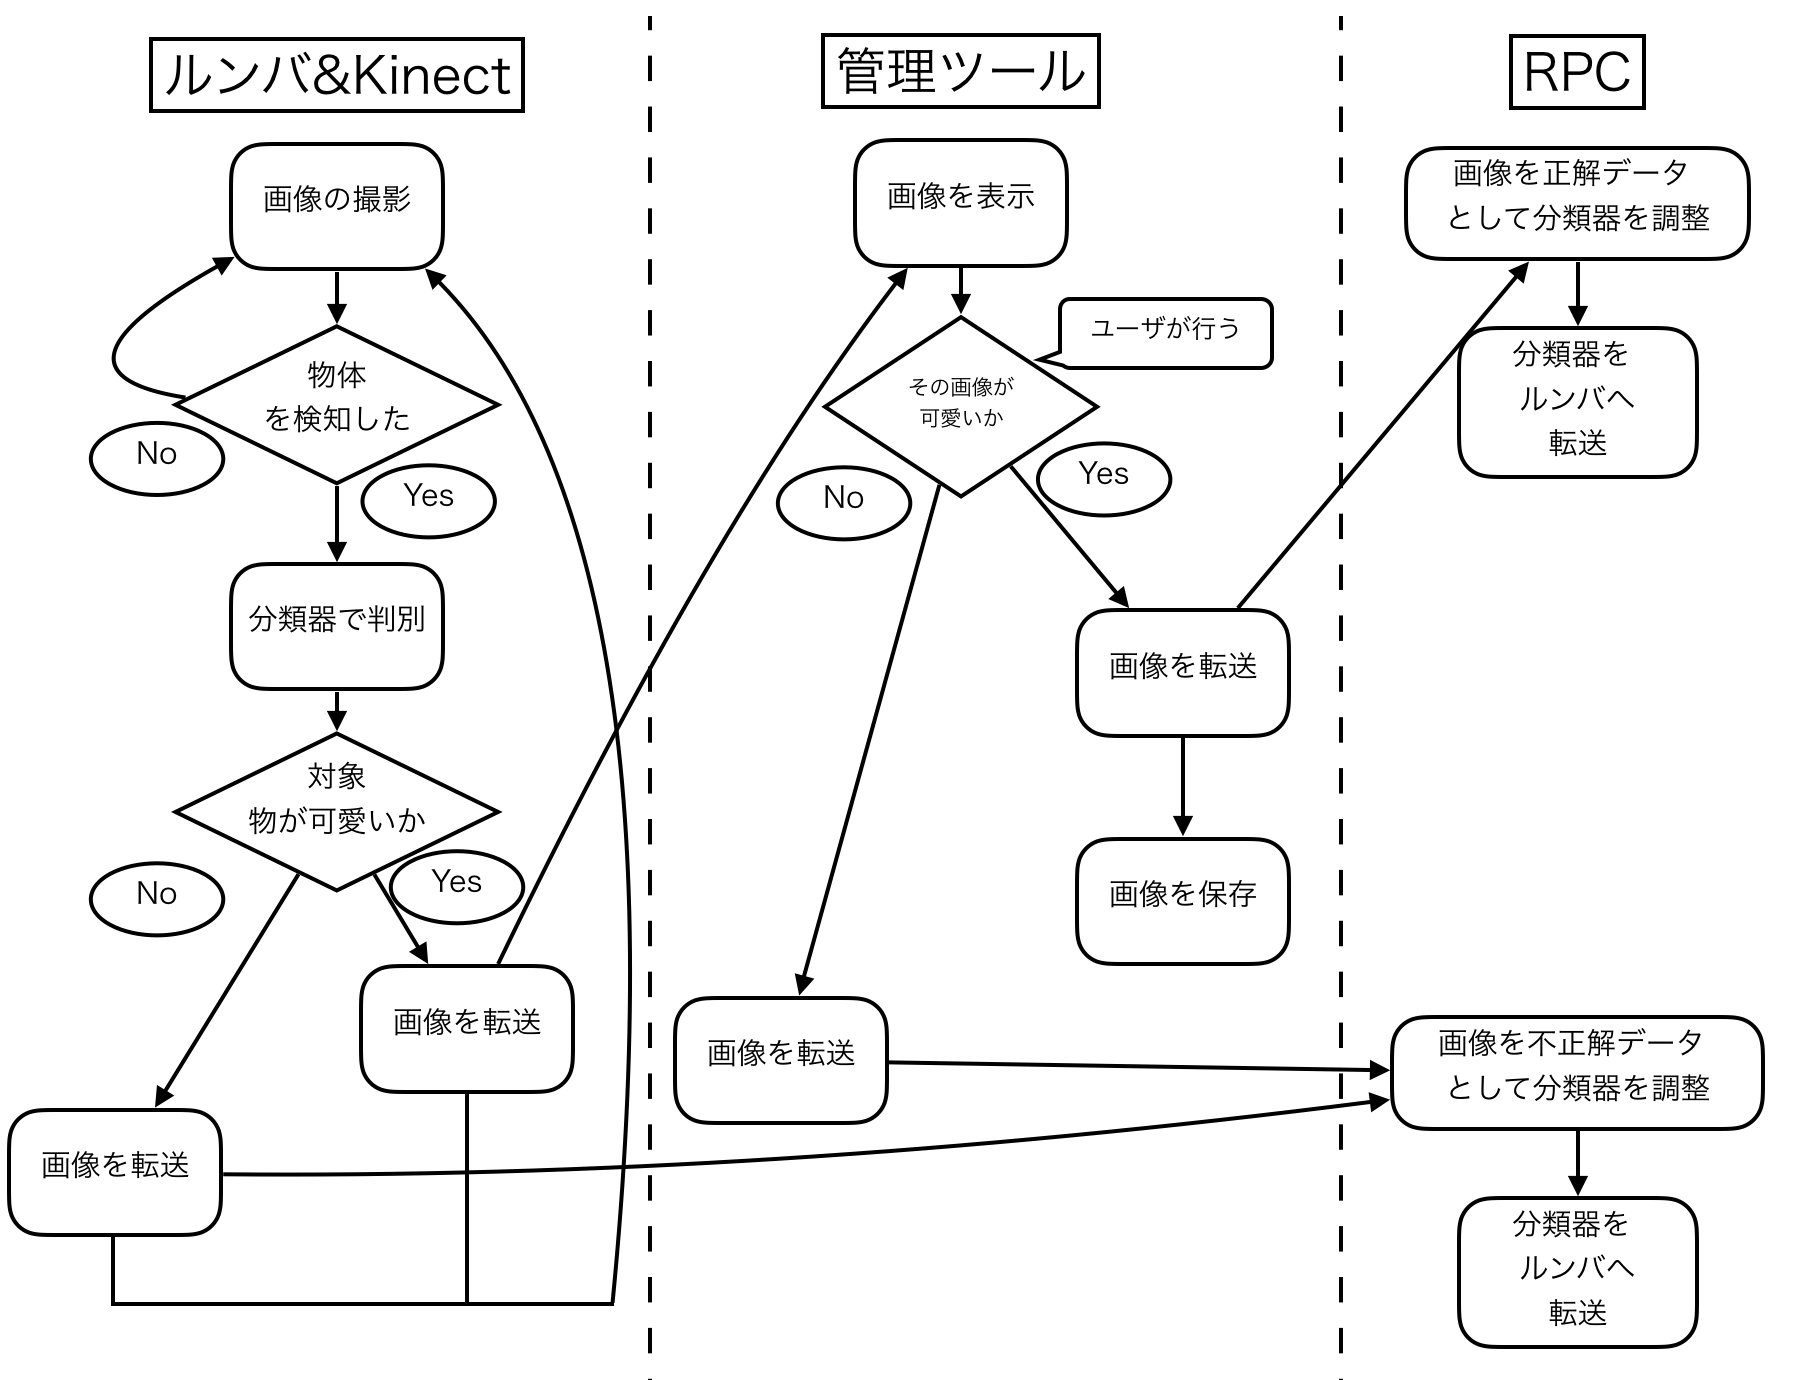
\includegraphics[width=8.5cm]{fig/flow_search.png}
	\caption{探索モードのフロー}
	\label{fig:search_flow}
\end{figure}

次に,本システムの作業フローについて説明する.
まず,学習モードの作業フローを図\ref{fig:learn_flow}に示す.
学習モードでは,本システムの利用者がルンバに対して命令を出す.
本システムの利用者はルンバが搭載しているKinectが映している映像を見ながら操作を行う.
その命令は前後の移動,左右の旋回,画像の撮影である.
命令が前後の移動,左右の旋回だった場合,ルンバは命令に従ってその動作を行う.
命令が画像の撮影であった場合,ルンバは現在映っている画像をRPCに転送し,その画像を正解データとして分類器の調整を行う.
次に,探索モードの作業フローを図\ref{fig:search_flow}に示す.
ルンバは搭載されている単純なアルゴリズムで対象物を探索する.
そして,物体が検出されるとその画像を保存し,分類器で判別を行う.
かわいいと判別された場合はその画像を管理ツールで表示し,利用者がその画像の判断を行う.
利用者がかわいいと判断した場合は,その画像をRPCに転送し,正解データとして分類器の調整を行い,かわいくないと判断した場合は,その画像をRPCに転送し,不正解データとして分類器の調整を行う.
分類器でかわいくないと判別された場合はその画像をRPCに転送し,不正解データとして分類器の調節を行う.

本稿では,RaspberryPiによるRPCの構築について説明する.

\section{アプローチ}
本節ではRPCの構築のアプローチを説明する.
この環境を構築するにはRaspberryPiを複数台接続し,分散的に処理を行う必要がある.
そこで,RPCではRaspberryPiで仮想マシンを起動し,仮想マシンを複製や移動によって柔軟な対応を取り,システムの性能や効率の向上を図る.
この手法はAmazon Web Service~(AWS)\cite{aws}やMicrosoft Azure\cite{azure}のようなクラウドサービスで用いられているため,まずはクラウド環境について説明する.

\begin{figure}[t]
	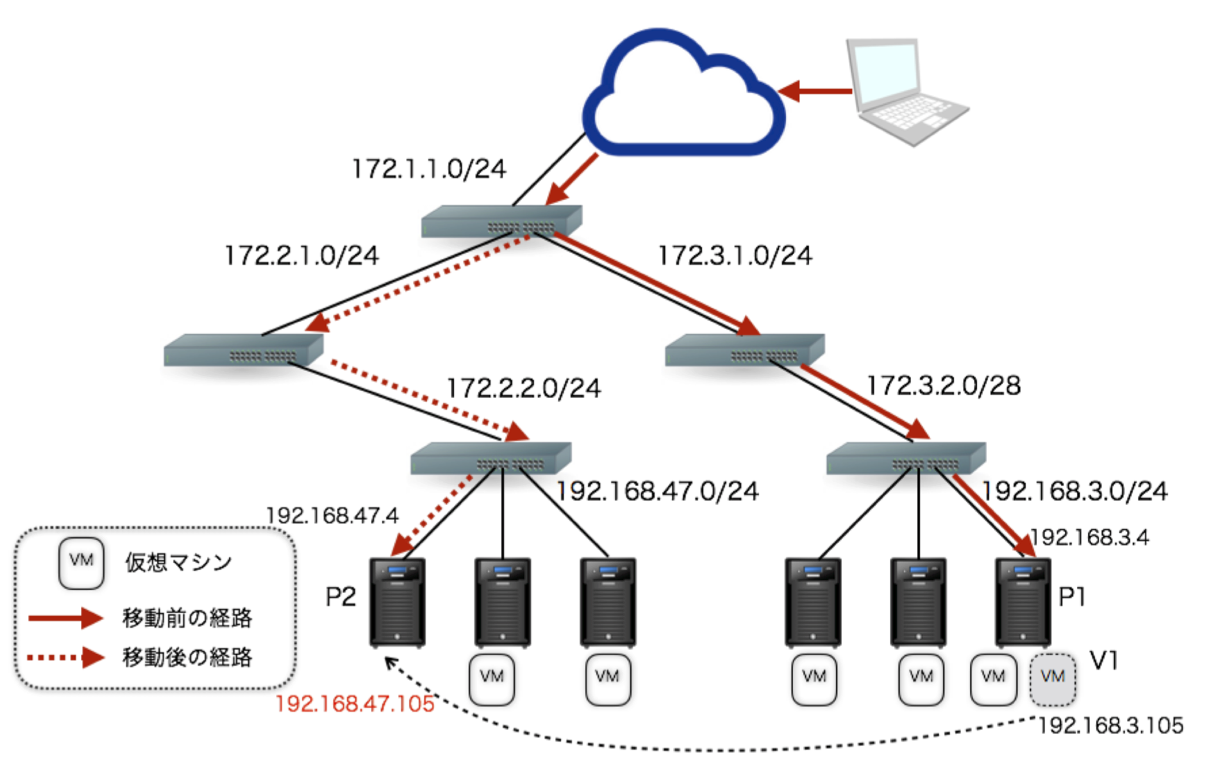
\includegraphics[width=8.5cm]{fig/cloud.png}
	\caption{想定するクラウド環境}
	\label{fig:cloud}
\end{figure}

\subsection{クラウド環境}
\label{subsec:cloud}
本システムで想定するクラウド環境を図\ref{fig:cloud}に示す.クラウド環境で
は,一般に複数のネットワークスイッチとそれらに接続した物理マシンで構成
される.そして,サービス提供者からリソース取得の要求があると,インフラ
提供者は物理マシンで仮想マシンを起動してそれらを提供している.クライア
ントのリクエストはスイッチで適切に転送され,対象となる仮想マシンが適切
に処理してサービスを運用している.ここで,物理マシンが高負荷になり,仮
想マシンが移動する状況を想定する~(図\ref{fig:cloud}).図
\ref{fig:cloud}では,物理マシンP1で仮想マシンV1が動作している状況にお
いて,V1を物理マシンP2に移動することを想定している.P1とV1にはそれぞれ
IPアドレス(192.168.3.4, 192.168.3.105)が設定されており,ユーザの立場か
らは区別できない.一方,P2にも192.168.47.4のIPアドレスが設定されている.
仮想マシンの移動では,一般にIPアドレスは変化しないため,V1のIPアドレス
はP2に移動した後も変わらず192.168.3.105となる.V1の移動はP2が直接接続
しているネットワークスイッチ,および上流に位置するスイッチに影響しない
ため,従来V1に届けられていたパケットは依然として192.168.3.0/24を管理す
るスイッチに届けられることになり,移動後のV1に届けられることはない.移
動後のV1に正しくパケットを届けるためには,V1のIPアドレスと移動後のネッ
トワークに合致したものに変更(e.g., 192.168.47.105)する必要がある.しか
しながら,ユーザがこの変更を知る手段がないため,V1へのリクエストは依然
として192.168.3.105宛に送信される.したがって,リクエストを正しく移動
後のV1に届けるためには,ネットワークスイッチに変更を加え,宛先
192.168.3.105へのパケットは変更後のアドレス(192.168.47.105)に書き換え
る必要がある.

このように,クラウド環境で円滑にサービスを運用するためには,仮想マシンの移動や
複製に伴い,関連するネットワークスイッチも連動して変更する必要がある.

\subsection{RPCの要件}\label{subsec:requirement}
\ref{subsec:cloud}節で述べたように,クラウド環境では仮想マシンの移動だけでなく,IPアドレスの変更など,移動に伴う変更や,移動の契機となる状況の把握,多数のマシンを制御する必要がある.
このことを踏まえて,本システムではRPCを実現するため,以下の項目を必要要件と考える.

\begin{description}
\item [負荷状況の把握]仮想マシンの移動や複製は,一般に高負荷状態にある
  物理マシンの負荷を分散し,仮想マシンで提供するサービスの性能維持や,
  低負荷状態の物理マシンに散財する仮想マシンを集約し,リソースの効率的
  な使用のために行われる.本環境でもこれらの負荷状態を測定する
  ため,負荷状態の判定に一般的に用いられるCPUとメモリ使用率を使用する.

\item [IPアドレスとルーティング管理]仮想マシンが移動する時,移動先物理マシンが同一
  ネットワークに所属している場合にはIPアドレスの変更は必要ない.しかし,
  \ref{subsec:cloud}節でも述べたように,異なるネットワークに所属する物
  理マシンに移動する場合には移動後にIPアドレスの変更が必要になる.同一
  ネットワーク内だけの移動/複製は,本システムの効率的な運用の妨げに
  なるため,本システムではネットワーク間を跨いだ仮想マシンの移動/複製も想定
  する.その場合,複数の物理/仮想マシンに同一のIPアドレスを指定するこ
  とはできないため,仮想マシン移動時にはIPアドレスを開放し,移動後には
  未使用のIPアドレスを設定する必要がある.
  さらに,ネットワーク間を跨いだ仮想マシンの移動/複製には,\ref{subsec:cloud}節で述べたように,
  IPアドレスの変更に伴い,関連するネットワークスイッチを変更し,適切にクライアントからのリクエストを 転送する必要がある.

\item [複数マシンの管理]本システムでは,多数の物理マシン,ネットワークスイッチで構成することになり,それぞれの状態管理(e.g, 負荷の測定)や制御(e.g, 設定変更や仮想マシンの移動/複製)を個別
  に行うことは現実的に難しい.そこで,本環境を構成する物理マシン
  やネットワークスイッチを一元管理し,設定変更や制御を自動で行う必要がある.
\end{description}

\section{設計}
本節では,RaspberryPiで仮想環境を実現する方法について述べ,それに際して必要となるネットワークを構築するOpenFlowについて述べる.
最後に,本システムの分散システムとしての要件をまとめる.

\begin{table}[t]
	\centering
	\caption{QEMUの機能}
	\label{tab:qemu_func}
	{
		\small
		\begin{tabular}{|c|c|} \hline
		qemu-img & 仮想マシンのイメージファイルの作成\\ \hline
		qemu-system-arm & 仮想マシンの起動\\ \hline
		migrate & 仮想マシンの移動\\ \hline
		\end{tabular}
	}
\end{table}

\subsection{RaspberryPIでの仮想化環境}
本環境では\ref{subsec:abstract}節で述べたように,RaspberryPI2 ModelBを利用する.CPUであるARM
Cortex-A7は仮想化拡張機能を備えているため,Linuxカーネルが備えるハイパー
バイザ,KVMを実行することができる.一般のPCでは,KVMはパッケージ管理ソ
フトウェア(e.g., apt-get)などを利用してインストールできるが,RaspberryPiでは
パッケージでは提供されていない.そのため,カーネルの組み込み機能として
実行する.また,KVMでの仮想マシンの管理にはvirt\cite{virt}を利用することが
一般的であるが,RaspberryPiではvirtを利用することができない\footnote{インストールは可能であるが,
実行できない}.そのため,本システムではKVMと連携して動作するqemu\cite{qemu}が提供する機能(表\ref{tab:qemu_func})を利用する.

一方,\ref{subsec:requirement}節でも述べたように,本システムの実現に
は仮想マシンの移動/複製に同期したネットワークの変更が必要になる.近年,
仮想化技術の進歩に伴い,ネットワークを柔軟に制御するためにSoftware
Defined Network~(SDN)\cite{sdn}が注目を集めており,利用されている.そ
こで本システムでもSDNを利用してネットワークを制御する.本研究ではSDNの一種
であり,広く利用されているOpenFlow\cite{opf}を利用するため,OpenFlow対
応のソフトウェアスイッチであるOpen vSwitch(OvS)をRaspberryPiにインストールし
て利用する.そのため,本環境はすべてRaspberryPiだけで構成できる.

\begin{figure}[t]
	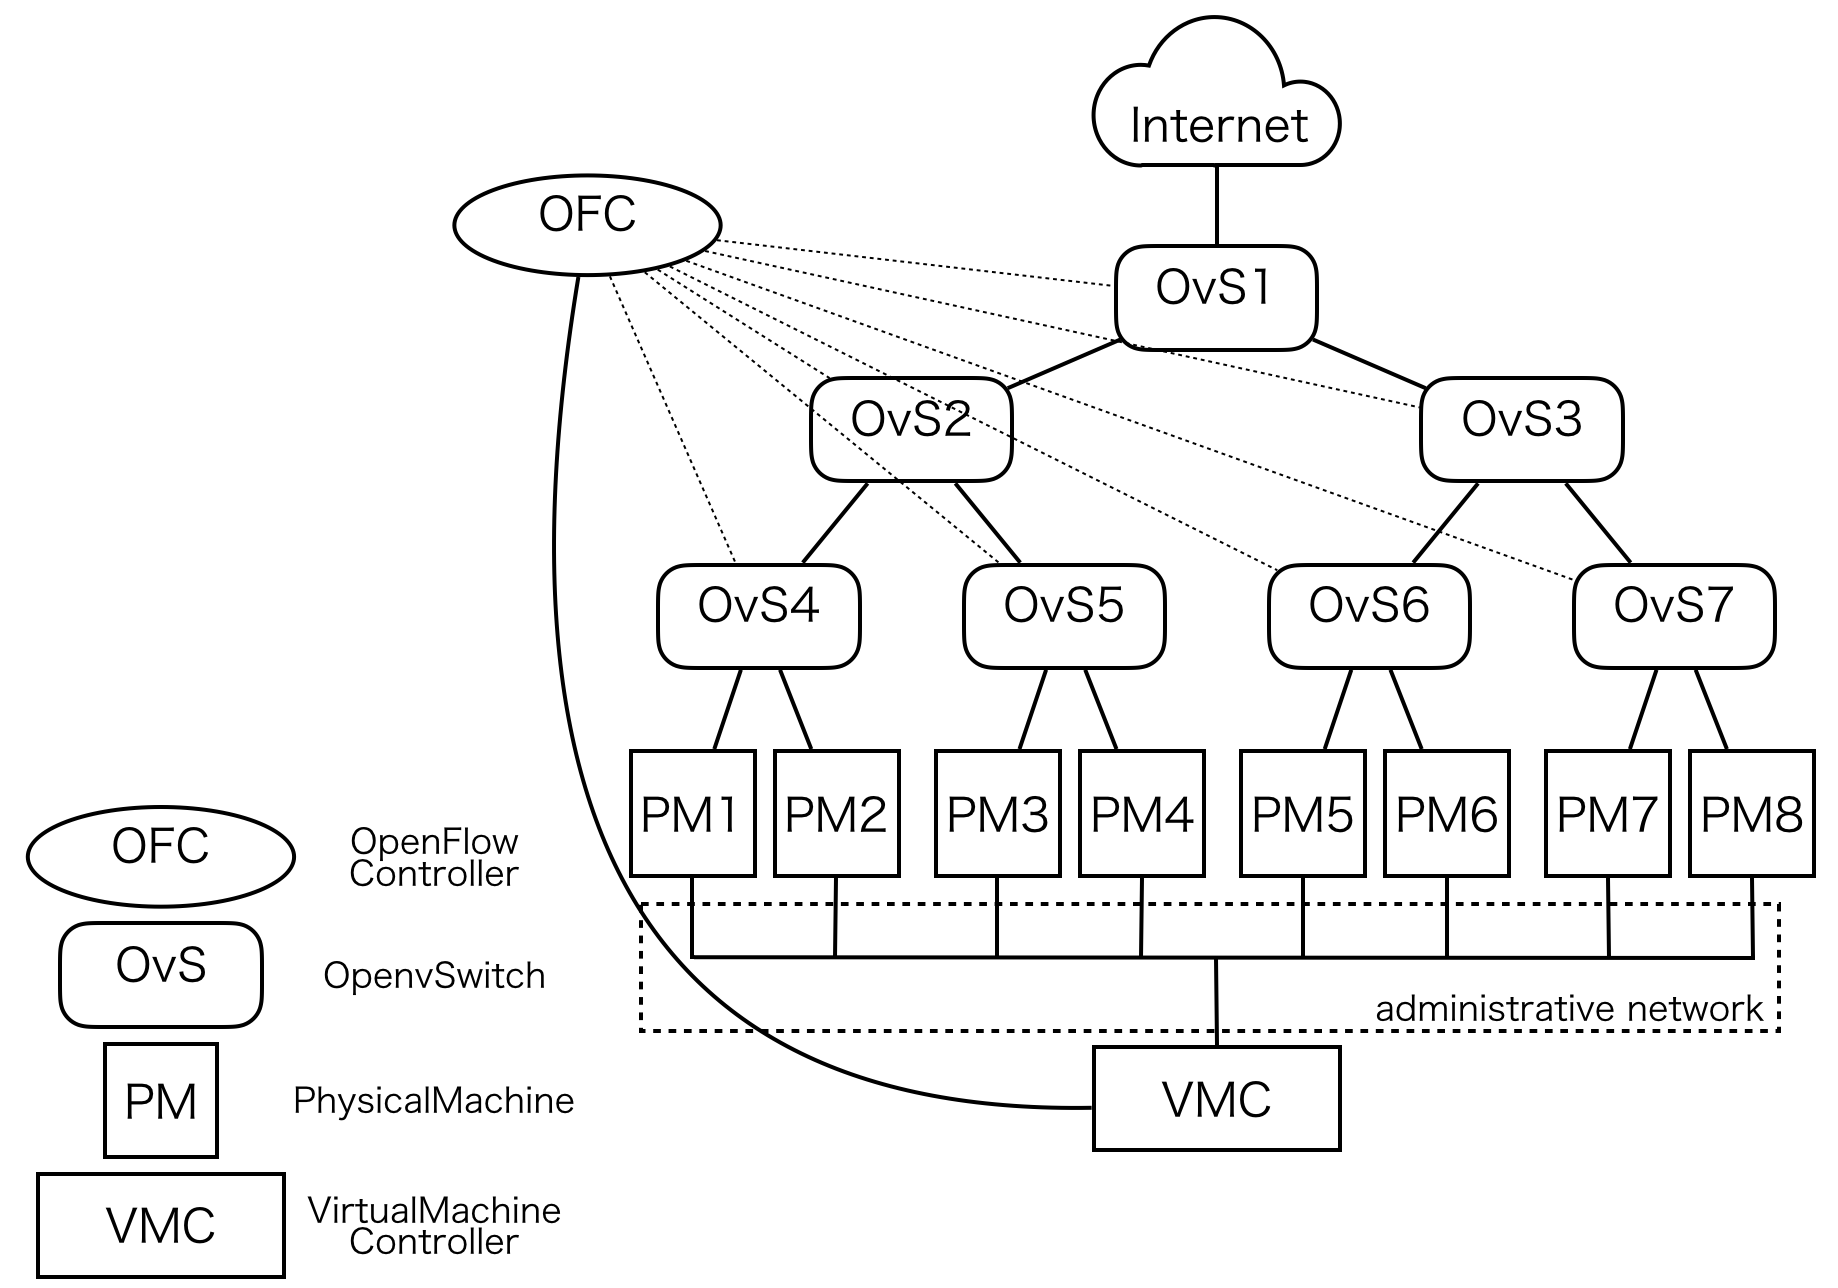
\includegraphics[width=8.0cm]{fig/topology.png}
	\caption{テスト環境のトポロジ}
	\label{fig:topology}
\end{figure}

\subsection{OpenFlowの概要}
SDNでは,経路制御を行うコントロールプレーンとデータの転送を行うデータ
プレーンが共存する既存のネットワーク機器とは異なり,コントロールプレー
ンとデータプレーンを分離したアーキテクチャを採用している.OpenFlow
は,データプレーンをOpenFlowスイッチと呼び,OpenFlowスイッチを制御す
るコントロールプレーンをOpenFlowController(OFC)と呼ぶ.  OpenFlowスイッ
チではデータの転送のみを行い,経路制御は OFCによって行われる.
OpenFlowスイッチは,パケットが内包する情報(送信元/送信先IPアドレスなど)を条件に
対象となるパケットを抽出し,それらに対して適切なアクション(パケット転送など)を実行する.
この,条件とアクションの組み合わせをフローと呼び,それらをまとめたテーブルをフローテーブルと呼ぶ.
OpenFlowスイッチはフローテーブルを保持し,自身がもつフローに従ってパケットを処理する.そして,
条件に合致しないパケットをOpenFlowが受信した場合,OpenFlowスイッチはOFCに問い合わせ(パケットイン),
適切なフローを受信してパケットを処理すると伴に,フローテーブルに記憶する.

\subsection{分散システムの要件}
本稿で説明したRPCにおいて,分散システムであることはシステムの効率を上げるために必要である.
RPCを実装するにあたって,必要となる分散システムの要件を以下に記述する.

まずは透過性について説明する.
\begin{description}
  \item[位置透過性]本システムでは,OpenFlowによるパケットの振り分けを行うため,ルンバは1つの仮想マシンのIPアドレスを知っていれば,各仮想マシンにパケットが振り分けられ処理を行うことができる.
  \item[移動透過性]仮想マシンの起動,複製,移動が行なわれるが,OpenFlowがパケットを書き換え,データの転送を行うので,ルンバは仮想マシンの状況を知る必要がない.
  \item[複製透過性]仮想マシンが(データごと)複製されるが,ルンバはそのことを考慮する必			  要がない.
  \item[並行透過性]リソース(機械学習の教師データなど)を複数の仮想マシンやユーザ間で共有することが可能である.
  \item[障害透過性]物理マシンの障害が発生しても,OpenFlowが検知し,その物理マシンを避けてデータの転送を行うので,ユーザには障害が発生していないように見える.
\end{description}

次にスケーラビリティについて述べる.
\begin{description}
  \item[サービス]複数仮想マシンでデータの処理を行うので,ユーザが増加してもシステムの運営には影響を与えない.
  \item[データ]新たにRaspberryPiを接続することで,物理的にリソースを増やすことが可能である.
  \item[アルゴリズム]OpenFlowで負荷状況に応じて負荷を分散することが可能である.
\end{description}

\section{実装}
本節では,\ref{subsec:requirement}節で挙げた要件に対応する本システムでの実現方法を述
べる.

\subsection{テスト環境のアーキテクチャ}\label{subsec:arch}
\ref{subsec:requirement}節で述べたように,多数の物理マシンや仮想マシンの
状態管理,および制御を個別に行うことは困難である.そこで,本システムでは,
仮想マシンや仮想マシンを起動する物理マシンを一元管理する仮想マシンコン
トローラ(VMC)を実現する.また,KVMを用いた仮想マシンの移動にはNFSを利
用する必要があり,一般にNFSの利用はローカルネットワークであることが望
ましい.そこで本システムでは,図\ref{fig:topology}に示すように,ユー
ザがサービス利用のために利用するネットワークとは異なる管理ネットワーク
を設け,すべての物理マシンを管理ネットワークにも接続する.そして,この
管理ネットワークにVMCを接続することで,後述する負荷状況やIPアドレス,
およびルーティングの管理を容易にする.

\begin{table}[t]
	\centering
	\caption{統計情報\cite{opf}}
	\label{tab:counters}
	\vspace{3mm}
	{
		\begin{tabular}{|l|c|} \hline
		カウンター & Bits \\ \hline \hline
		\multicolumn{2}{|c|}{フローテーブルごと} \\ \hline
    有効エントリー数 & 32 \\
    パケットルックアップ数 & 64 \\
    パケットマッチ数 & 64 \\ \hline
		\multicolumn{2}{|c|}{フローごと}\\ \hline
    受信パケット数 & 64 \\
    受信バイト数 & 64 \\
    フローが作られてからの経過時間(秒) & 32 \\
    フローが作られてからの経過時間(ナノ秒) & 32 \\ \hline
		\multicolumn{2}{|c|}{ポートごと} \\ \hline
    受信パケット数 & 64 \\
    転送パケット数 & 64 \\
    受信バイト数 & 64 \\
    転送バイト数 & 64 \\
    受信ドロップ数& 64 \\
    転送ドロップ数& 64 \\
    受信エラー数 & 64 \\
    受信フレームアライメントエラー数 & 64 \\
    受信オーバーランエラー数 & 64 \\
    受信CRCエラー数 & 64 \\
    コリジョン数 & 64 \\ \hline
    \multicolumn{2}{|c|}{キューごと} \\ \hline
    転送パケット数 & 64 \\
    転送バイト数 & 64 \\
    転送オーバーランエラー数 & 64 \\ \hline
		\end{tabular}
	}
\end{table}

\subsection{負荷状況の把握}
負荷状況の指標となる各物理マシンのCPUとメモリ使用率,各スイッチのトラ
フィック量を取得する.CPUとメモリ使用率の取得には,各物理マシンの/proc
ディレクトリ以下に格納される情報(meminfo)を利用し,一定間隔(現在は10
秒)で継続的に取得する.また,トラフィック量の取得には,表
\ref{tab:counters}で示すOvSが保持する統計情報を利用し,各OvS単位,およ
び個々のOvSのポート単位でのトラフィック量を計測する.これらの情報を
OFCに集約し,VMCと連携する.

\subsection{IPアドレスとルーティング管理}
\label{subsec:ip_routing}
\ref{subsec:cloud}節で述べたように,クラウド環境の実現には仮想マシンの
移動や複製だけでなく,関連するネットワークスイッチも連動して変更する必
要がある.そのため,本システムでは仮想マシンに使用するIPアドレスは
DHCPを用いることなくVMCが管理し,仮想マシンの移動に同期した変更を可能
にする.本システムでは,仮想マシンに付与するIPアドレスのネットワーク
アドレスは,物理マシン所属するネットワークアドレスと同一である必要があ
る.そのため,移動や複製に伴い変更の必要がある.本システムでは,使用
中のIPアドレス,ネットワークアドレスをVMCで集中管理しており,仮想マシ
ンの移動や複製先のネットワークに適したIPアドレスを付与する.仮想マシン
への具体的な設定は,ifconfigやrouteコマンドを使用したスクリプトを用意
している.

次に,\ref{subsec:cloud}節で述べたように,クライアントのリクエストを正
しく移動,または複製後の仮想マシンに届けるためには,リクエストを経由す
るスイッチを適切に変更する必要がある.
VMCは仮想マシンの移動または複製を行った後,移動・複製前,および
移動・複製後のIPアドレス,実行の種類(移動または複製)をOFCに通知する.
OFCは関連するOvSを特定し,適切に設定変更する必要がある.
以降,同一ネットワーク,およびネットワークを跨いで仮想マシンが
移動または複製されるときの設定変更について述べ,最後に関連するOvSの特
定について述べる.

\begin{figure}[t]
	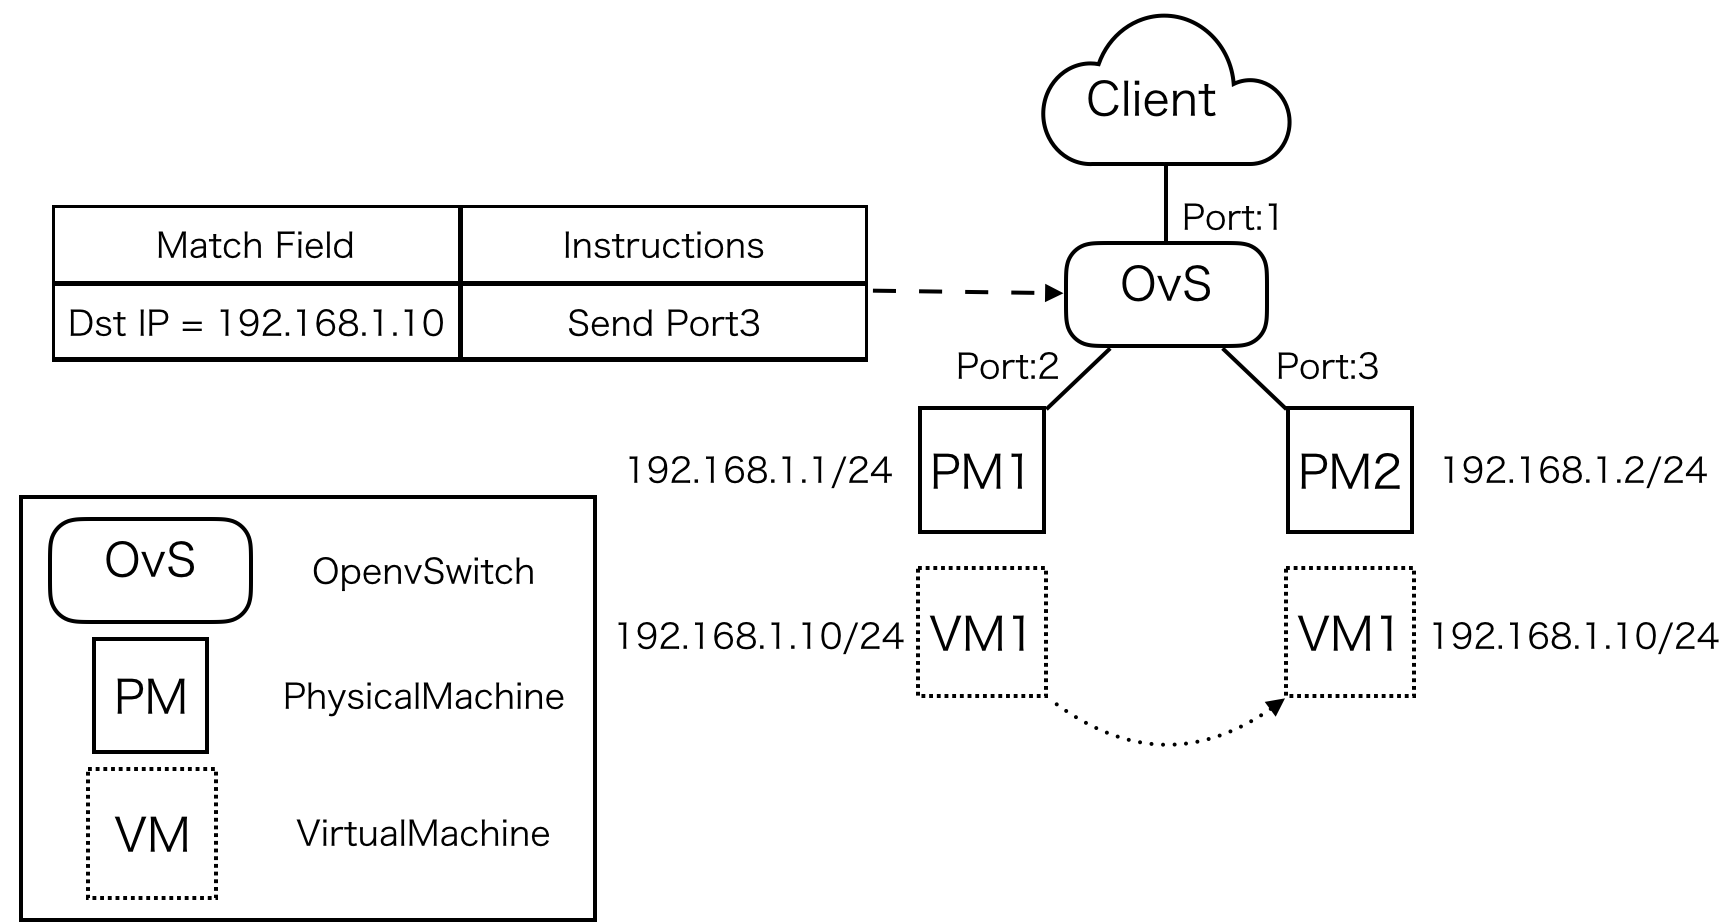
\includegraphics[width=8.5cm]{fig/migrate_flow.png}
	\caption{同一ネットワークへの仮想マシンの移動}
	\label{fig:migrate_flow}
\end{figure}
\begin{figure}[t]
	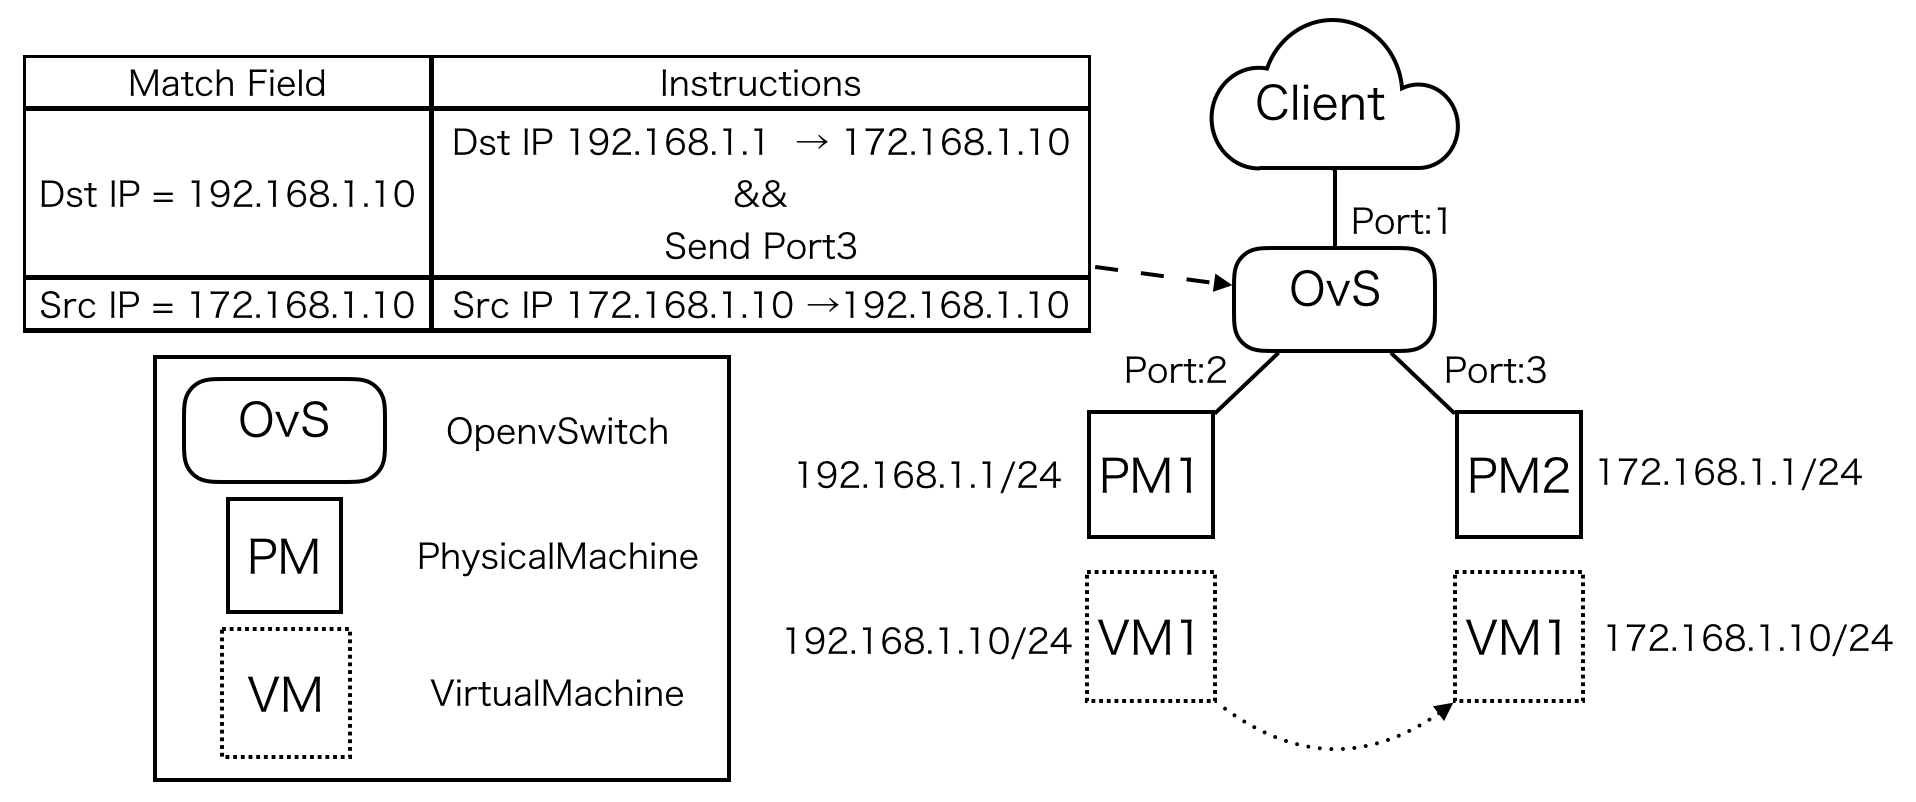
\includegraphics[width=8.5cm]{fig/migrate_flow_diff.png}
	\caption{外部ネットワークへの仮想マシンの移動}
	\label{fig:migrate_flow_diff}
\end{figure}
\begin{figure}[t]
	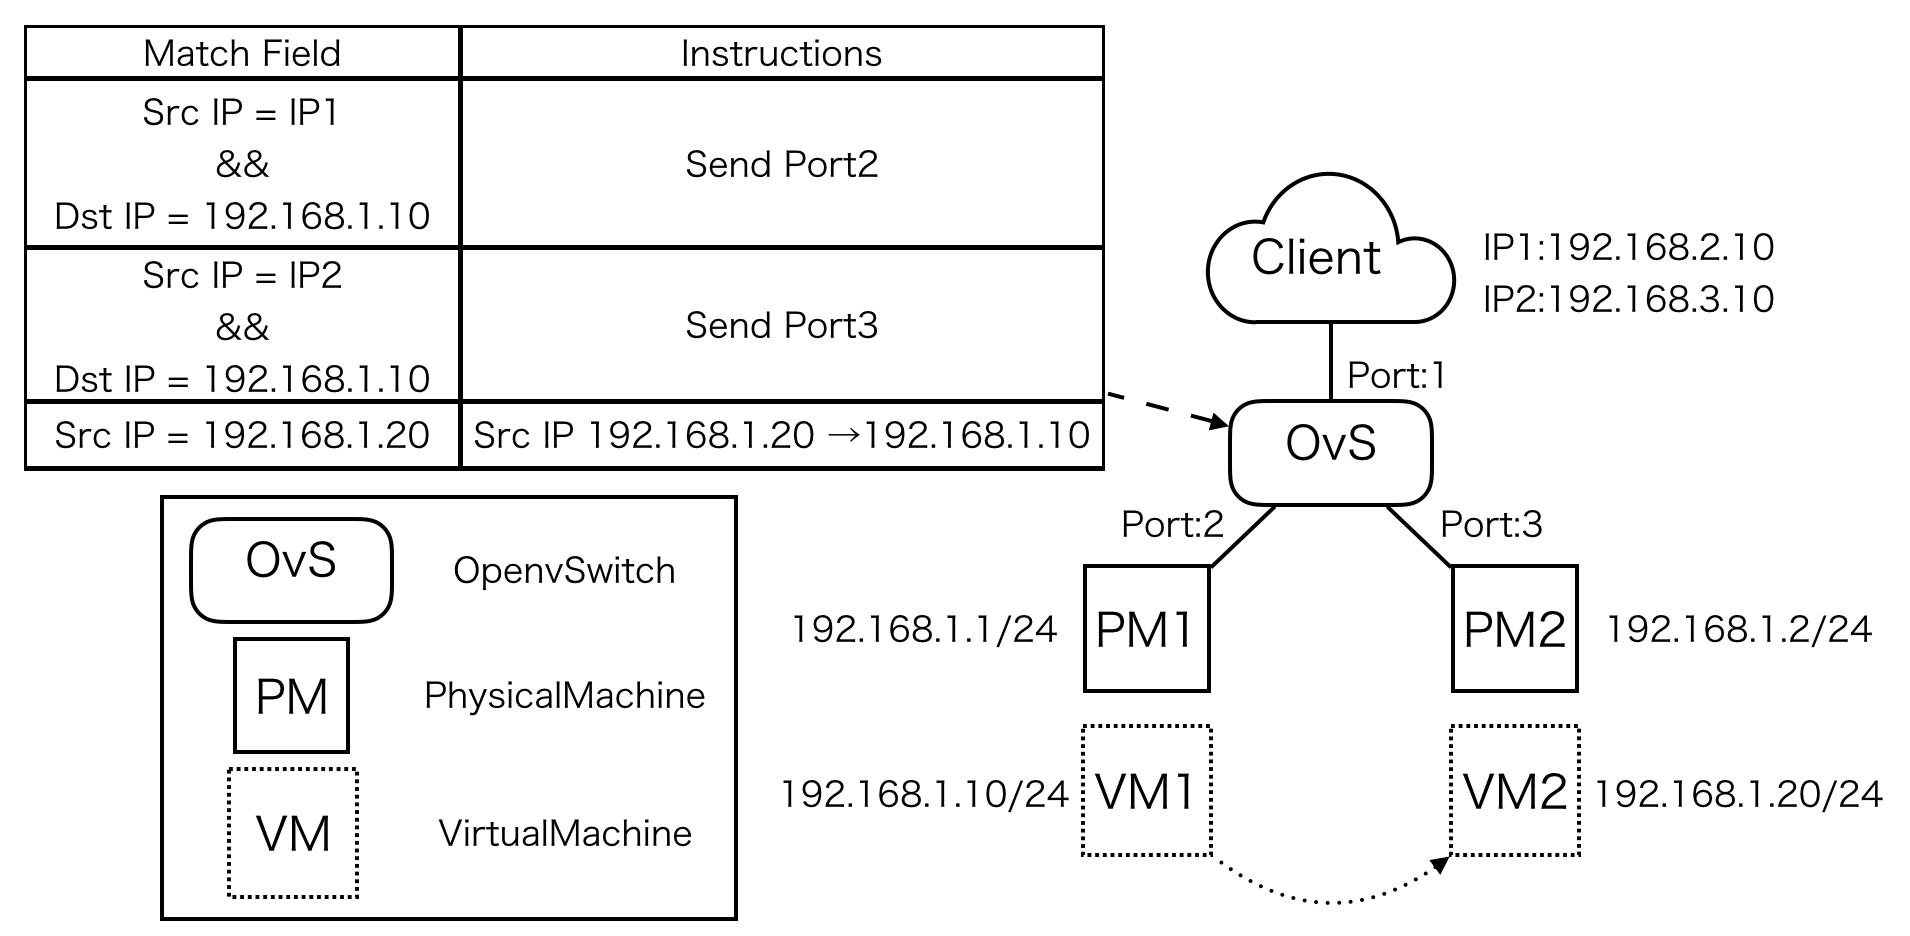
\includegraphics[width=8.5cm]{fig/clone_flow.png}
	\caption{仮想マシンの複製}
	\label{fig:clone_flow}
\end{figure}

\begin{enumerate}
 \item 同一ネットワークへの仮想マシンの移動\\同一ネットワーク内の仮想
   マシンの移動ではIPアドレスの変更は行われない.したがって,図
   \ref{fig:migrate_flow}に示すように,特定したOvSにおいて,転送先アド
   レスがVM1(192.168.1.10)にマッチしたパケットの送出ポート番号を変更す
   る(Port2 $\rightarrow$ Port3).

 \item 外部ネットワークへの仮想マシンの移動\\外部ネットワークへの仮想
   マシンの移動では,IPアドレスの変更が伴う.図
   \ref{fig:migrate_flow_diff}では,異なるネットワークに所属するPM1と
   PM2間で仮想マシンが移動する.そこで,OvSでは転送先アドレス
   192.168.1.10にマッチしたパケットの送出ポートを変更し(Port2
   $\rightarrow$ Port3),かつパケットのDSTアドレスを変更する
   (192.168.1.10 $\rightarrow$ 172.168.1.10).さらに,172.168.1.10から
   の送信元に戻されるパケットについては,OvSでSRCアドレスを
   192.168.1.10に書き換える.その結果,クライアントが仮想マシンの移動
   に気づくことはない.

 \item 仮想マシンの複製\\仮想マシンが複製される場合,同一ネットワーク
   か否かに関わらず,複製した仮想マシンには新たなIPアドレスが割り当て
   られ,仮想マシン間でリクエストを分散して処理する.このとき,複製前
   に既にリクエストを処理したクライアントに対しては複製前の仮想マシン
   がリクエストを処理し,新たにリクエストを送信したクライアントに関し
   てはラウンドロビンで処理を分散する.

   図\ref{fig:clone_flow}は2台のクライアント(IP1, IP2)のうちIP1が
   VM1(192.168.1.10)に既にアクセスしており,VM2(192.168.1.20)を生成後,
   IP2がVM1に対してリクエストを送信したときの様子を示している.IP1から
   VM1へのリクエストは既に実行されているため,IP1からVM1へのリクエスト
   はOvSのフローテーブルに従って引き続きPort2に送出される.一方,IP2か
   らVM1へのリクエストはOvSのフローテーブルにマッチしないため,OvSは
   OFCに処理の問い合わせを行う(パケットイン).この時,OvSはVMCによって
   複製されたVM2のIPアドレスを認識しているため,パケットのDSTアドレス
   を変更する(192.168.1.10 $\rightarrow$ 192.168.1.20)してPort3に送出
   する.そして,学部ネットワークへ仮想マシンの移動と同様,戻りパケッ
   トのSRCアドレスをVM1のものに書き換える(192.168.1.10).
   その結果,処理の分散はクライアントには透過であり,既存のクライアント(IP1)
   のセッションも維持される.

\end{enumerate}

\subsection{複数マシンの管理}
\ref{subsec:arch}で述べた通り,VMCを使用することで,多数の物理マシンや仮想マシンの状態管理や制御を個別に行うことが可能になる.
本システムの利用者はそのサーバにアクセスすることで本環境の設定を行うことができる.
各物理マシン,仮想マシンのIDやリソース状況はhostname/indexで確認することができる.
この情報を元に,リソースの閾値や仮想マシンの管理を行い,システムを自動で効率よく運用できるとともに,システム利用者が予測していなかった状態でも管理することができる.

\section{評価・考察}
本節では,RaspberryPi 17台(OvSに7台,PMに8台,OFCとVMCにそれぞれ1台)を使用し
て図\ref{fig:topology}に示すトポロジを構成し,本システムを評価する.

まず,RaspberryPiでのOpenFlow環境が十分な性能を有すること
を示すため,複数のOvSを経由するときのトラフィック量を計測し,スループッ
トを示す.次に,仮想マシンの移動,および複製時の実行時間を測定して
本テスト環境の基本性能を示す.次に,仮想マシンの移動,複製時,時間経
過に伴うのCPUとメモリ使用率を測定し,考察する.最後に,RaspberryPiで分類器の作成を行なった時にどのようなリソース推移になるかの結果を提示し,考察する.

\begin{table}[t]
	\centering
	\caption{サーバを通信する時の経由するOvSの数}
	\label{tab:route}
	\vspace{4mm}
	{
		\begin{tabular}{ c c c } \hline
      route & 通信間 & 経由するOvS数 \\ \hline \hline
      1 & PM1 $\longleftrightarrow$	PM2 & 1 \\ \hline
      2 & Internet $\longleftrightarrow$ PM1 & 3 \\ \hline
      3 & PM1 $\longleftrightarrow$	PM3 & 3 \\ \hline
      4 & PM1 $\longleftrightarrow$	PM8 & 5 \\ \hline
		\end{tabular}
	}
\end{table}

\begin{figure}[t]
	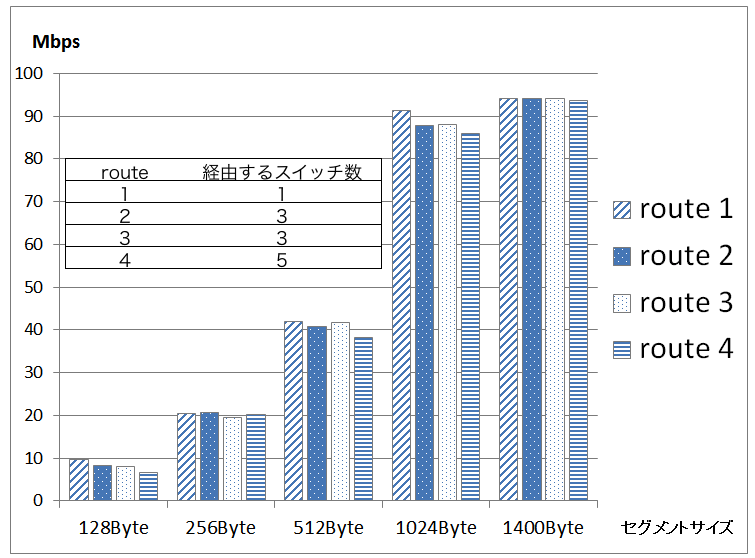
\includegraphics[width=8.5cm]{fig/graph.png}
	\caption{ネットワーク速度}
	\label{fig:graph}
\end{figure}

\subsection{RaspberryPiでのOpenFlow環境}
RaspberryPiを用いたOvSのスループットを測定するため,図\ref{fig:topology}に示
すトポロジにおいて,表\ref{tab:route}に示す経路でネットワークに負荷を
かけ,スループットを計測する.この計測にはiperf\cite{iperf}を利用し,
最大TCPセグメントを,128/256/512/1024/1400[Byte]としたときの値を測定し
た.まず,設定した最大TCPセグメントに依存せず,route1とroute4を比較す
ると分かるように,経由するOvSの数によって僅かに転送速度が低下する.こ
れは,パケット転送に関連するOvSの個数の影響であり,最大でも5Mbps程度の
性能低下であることから(最大TCPセグメントサイズ1024[Byte]の場合),極端
な速度低下は見られない.
また,最大TCPセグメントサイズを2倍にするごとににスループットも倍増していることから,
パケット転送に関しては十分な性能が得られていることがわかる.なお,最大TCPセグメントサイズ
が1400[Byte]の場合,1024[Byte]の場合と比較して大幅なスループットの向上は見られなれなかった.
これは,RaspberryPiのイーサネットポートが10/100Mbps対応であり,100Mbps以上のスループットを得られないためである.
一方,各OvSでは表\ref{tab:counters}で示した情報を取得できるため,
関連するOvSのトラフィック量を計測した.その結果,計測したトラフィック量の合計がiperfで転送したトラフィック量と一致することを確認した.

これらの結果から,RaspberryPiでのOpenFlow環境は十分な性能が得られると判断することができる.

\begin{table}[t]
	\centering
	\caption{仮想マシンの操作に要する時間}
	\label{tab:func_time}
	\vspace{4mm}
    \scalebox{1.0}
	{
		\begin{tabular}{|c|c|c|c|} \hline
            仮想マシンの操作& 起動(秒) & 移動(秒) & 複製(秒) \\ \hline \hline
            実行時間 & 47 & 32 & 49 \\ \hline
            ネットワーク構成変更 & & 3 & 4 \\ \hline
	  	\end{tabular}
	}
\end{table}

\begin{table}[t]
	\centering
	\caption{表\ref{tab:func_time}の実行時間内訳}
	\label{tab:func_breakdown}
	\vspace{4mm}
    \scalebox{1.0}
	{
		\begin{tabular}{|c|c|c|c|} \hline
            仮想マシンの操作& 起動(秒) & 移動(秒) & 複製(秒) \\ \hline \hline
						Qemuの機能 & 32 & 23 & 32 \\ \hline
						スナップショットの転送 & - & 2 & 2 \\ \hline
						ネットワークの設定 & 8 & - & 8 \\ \hline
						リソースの取得 & 7 & 7 & 7 \\ \hline
            合計 & 47 & 32 & 49 \\ \hline
	  	\end{tabular}
	}
\end{table}

\subsection{仮想マシンの移動と複製}
\label{subsec:migrate_duplicate}
本テスト環境では,仮想マシンの起動にqemuのスナップショット機能
\cite{snapshot}を用いている.また,この機能は仮想マシンの複製時にも利
用する.そのため,仮想マシンの移動と複製に加え,スナップショットを用い
た起動時間を表\ref{tab:func_time}に示し,その内訳を表
\ref{tab:func_breakdown}に示す.

表\ref{tab:func_breakdown}に示すように,仮想マシンの起動は,$a$)スナッ
プショットファイルを指定したqemu-system-armコマンドの実行,
$c$)ifconfigやrouteコマンドを利用した,ネットワーク設定用スクリプト
の実行(ネットワークの設定),$d$)仮想マシンのリソース使用量を測定するスクリプトの実行(リソースの取得),
で構成される.表\ref{tab:func_breakdown}より,仮想マシンの起動には$a$)
に32秒,$c$)に8秒,$d$)に7秒要し,起動して使用可能になるまでに約47秒か
かった.一方,仮想マシンの移動には,$a'$)migrateコマンドの実行,$b$)ス
ナップショットの転送,$d$)リソースの取得,で構成され,$a'$)に23秒,$b$)
に2秒,$d$)に7秒要し,移動全体で32秒要した.なお,この実験では仮想マシ
ンは同一ネットワーク内を移動したため,$c$)ネットワークの設定は必要ない.

最後に,仮想マシンの転送は,仮想マシンの起動に加えスナップショットの転送が加わるため,
$a$), $c$), $d$)の実行に加え,b)スナップショットの転送に2秒要し,全体で49秒要した.

これら3つの結果から,起動や移動で用いるコマンドの違いによって$a$)と$a'$)で
は必要な時間が異なるが,$b$), $c$), $d$)に要する時間はどの場合でも同じ値を示
した.これらのことから,本テスト環境で実現した機能($b$), $c$), $d$))は,安定
して動作すると考えることができる\footnote{VMCやOFCと各PM間の通信,およびスナップショット転送は
管理ネットワークを使用するため,安定したスループットを得られる.}.

一方,\ref{subsec:ip_routing}節で述べたように,仮想マシンの移動と複製
には,VMCがそれらの完了を検知した後,OFCに依頼して関連するOvSを変更す
る,というネットワーク構成変更を伴う.したがって,表
\ref{tab:func_time}に示すように,仮想マシン移動時にはネットワーク構
成変更に伴いクライアントのリクエストが3秒間遮断されたが,複製では遮
断されることなく通信することができた.これは,仮想マシン移動時は構成変
更が終わるまでパケットを受け取る仮想マシンが存在しなくなるのに対し,仮
想マシンの複製では複製後の仮想マシンに関するネットワークの変更が行われ
るまでは複製元の仮想マシンにリクエストが届けられていることを意味してい
る.

この結果から,本テスト環境で提供するネットワーク構成変更は正しく機能していると推察される.

\subsection{CPUとメモリ使用率の変化}
仮想マシンの起動,移動,および複製することによる物理マシンのリソース使
用率の変化を確認するため,物理マシンで仮想マシンを起動した後,2台の物
理マシン間で仮想マシンの移動,および複製するときのリソース使用率の変化
を確認する.また,仮想マシンの移動では,ネットワーク構成変更とリソース
使用率の変化も確認するため,仮想マシンでApacheを起動し,InternetからそのApacheにHTTPリ
クエストを送り続けながら仮想マシンを移動した.
\ref{subsec:migrate_duplicate}節で述べたように,移動や複製には管理ネッ
トワークを使用するため,移動や複製がネットワークを跨ぐ場合でも結
果に影響しない.そこで,本実験では図\ref{fig:topology}のPM1からPM2に仮
想マシンを移動,および複製した.仮想マシンを移動,および複製したときの
リソース使用率の変化を図\ref{fig:graph_migrate}, 図
\ref{fig:graph_clone}にそれぞれ示す.

まず,仮想マシンの移動では,PM1で仮想マシンが実行され,約40秒かけて起
動が完了する(図\ref{fig:graph_migrate}, 20から60秒付近).その間,CPUとメ
モリ使用率は上昇し,起動完了後にCPU使用率は再び仮想マシン起動前と同等
の値(10\%弱)を示している.この起動時間は表\ref{tab:func_breakdown}とほぼ一
致しており,リソース使用率の変化を正しく計測できていることを示唆してい
る.その後,HTTPアクセスを開始後,仮想マシンの移動が完了するまでCPU使
用率は平均20\%弱を示しており,HTTPリクエストの処理やmigrateコマンドの
実行に割り当てられていることがわかる.その後,仮想マシンの移動が完了
(図\ref{fig:graph_migrate},110秒付近)するとCPU使用率は再び仮想マシン起動前と同等の
値となった.また,メモリ使用率も仮想マシン移動後は仮想マシン起動前と同
等の値となった.

一方,仮想マシンの移動先であるPM2は,PM1でmigrateコマ
ンドが実行された時刻付近からメモリ使用率が上昇し始め,移動が完了するとCPU使用率
が上昇した.これは,PM2に仮想マシンが移動し,実行を開始したことを示唆
している.なお,PM2では仮想マシン移動完了後CPU使用率が急上昇した後,一
度下降しているが,これはネットワーク構成変更によってHTTPリクエストが届
かず,CPUはリクエストを処理していないことを示唆している.この振る舞い
は表\ref{tab:func_time}の結果とほぼ一致しているため,リソース使用率の変
化を正しく計測できていると考えることができる.

\begin{figure}[t]
	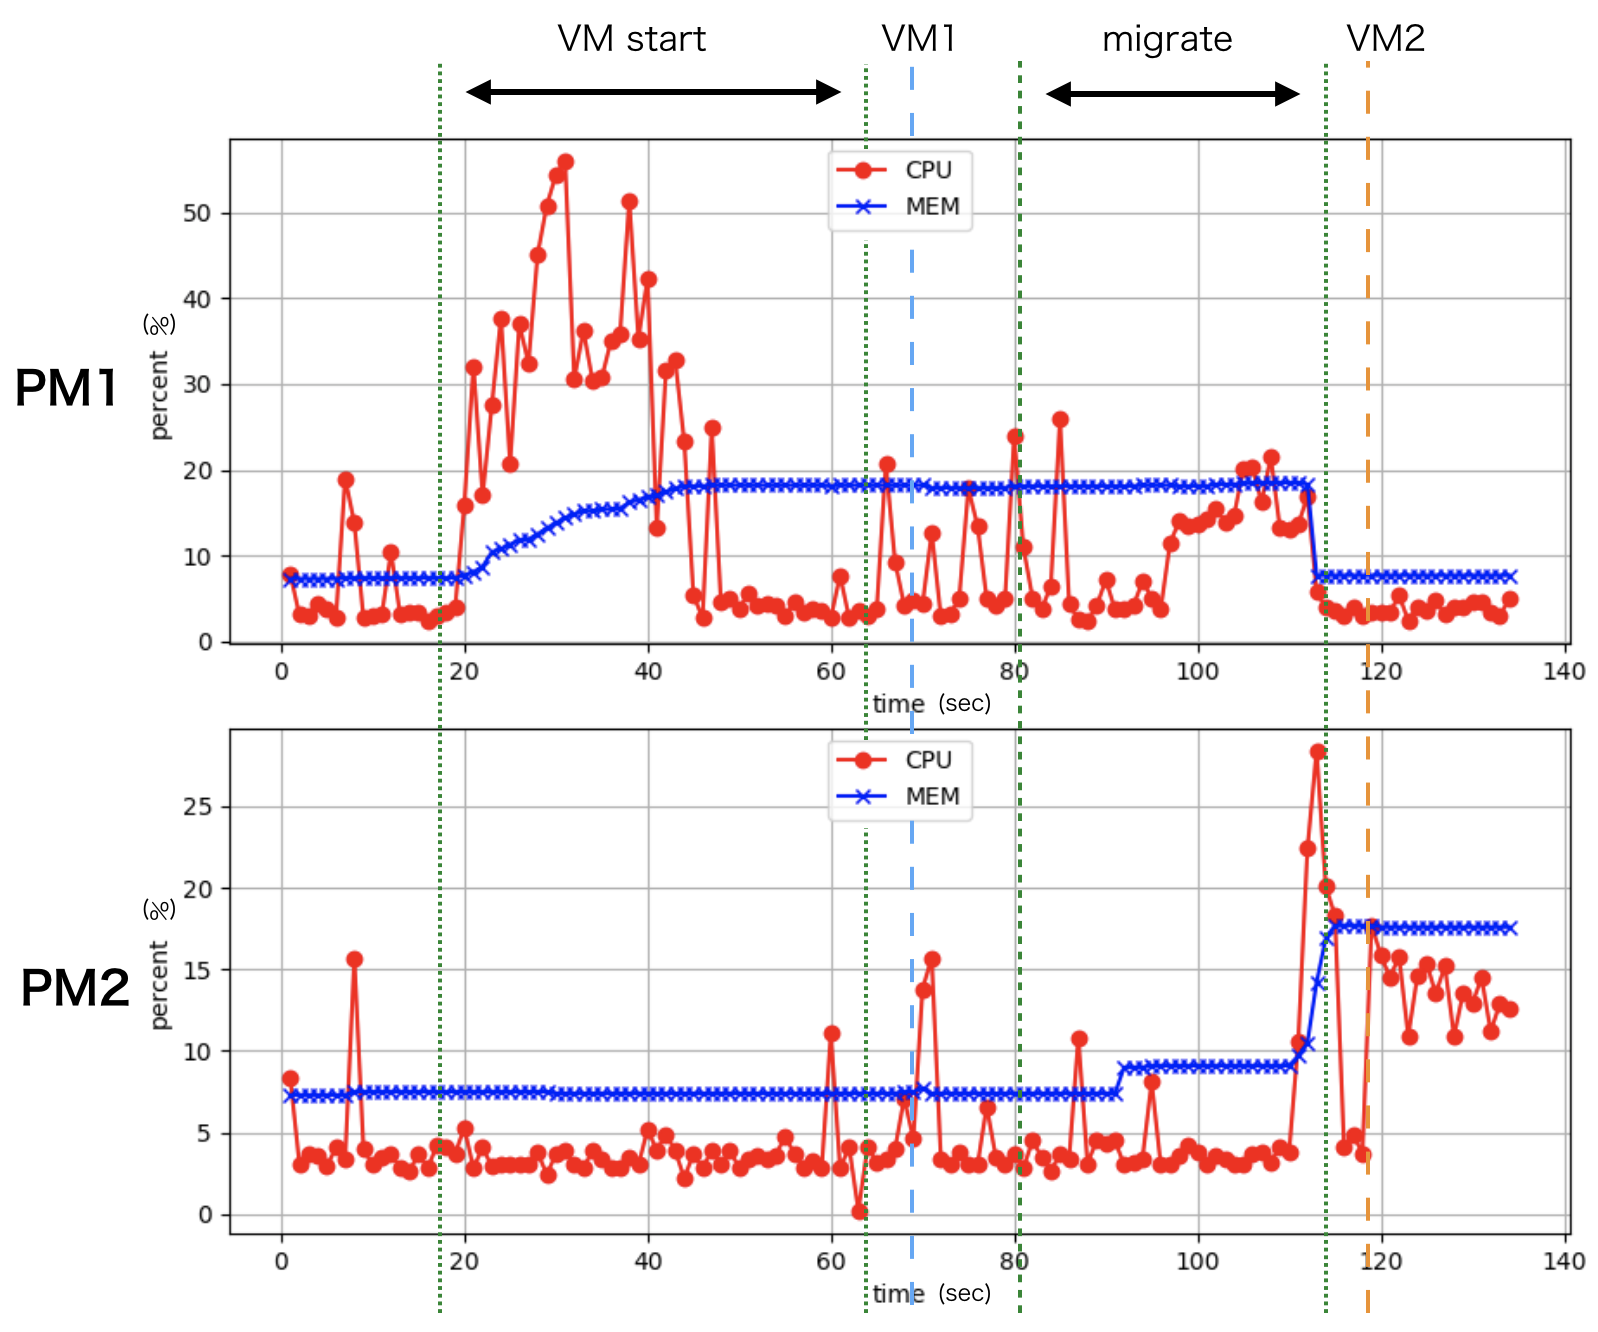
\includegraphics[width=9.0cm]{fig/migrate.png}
	\caption{仮想マシンの移動によるリソース推移}
	\label{fig:graph_migrate}
\end{figure}

\begin{figure}[t]
	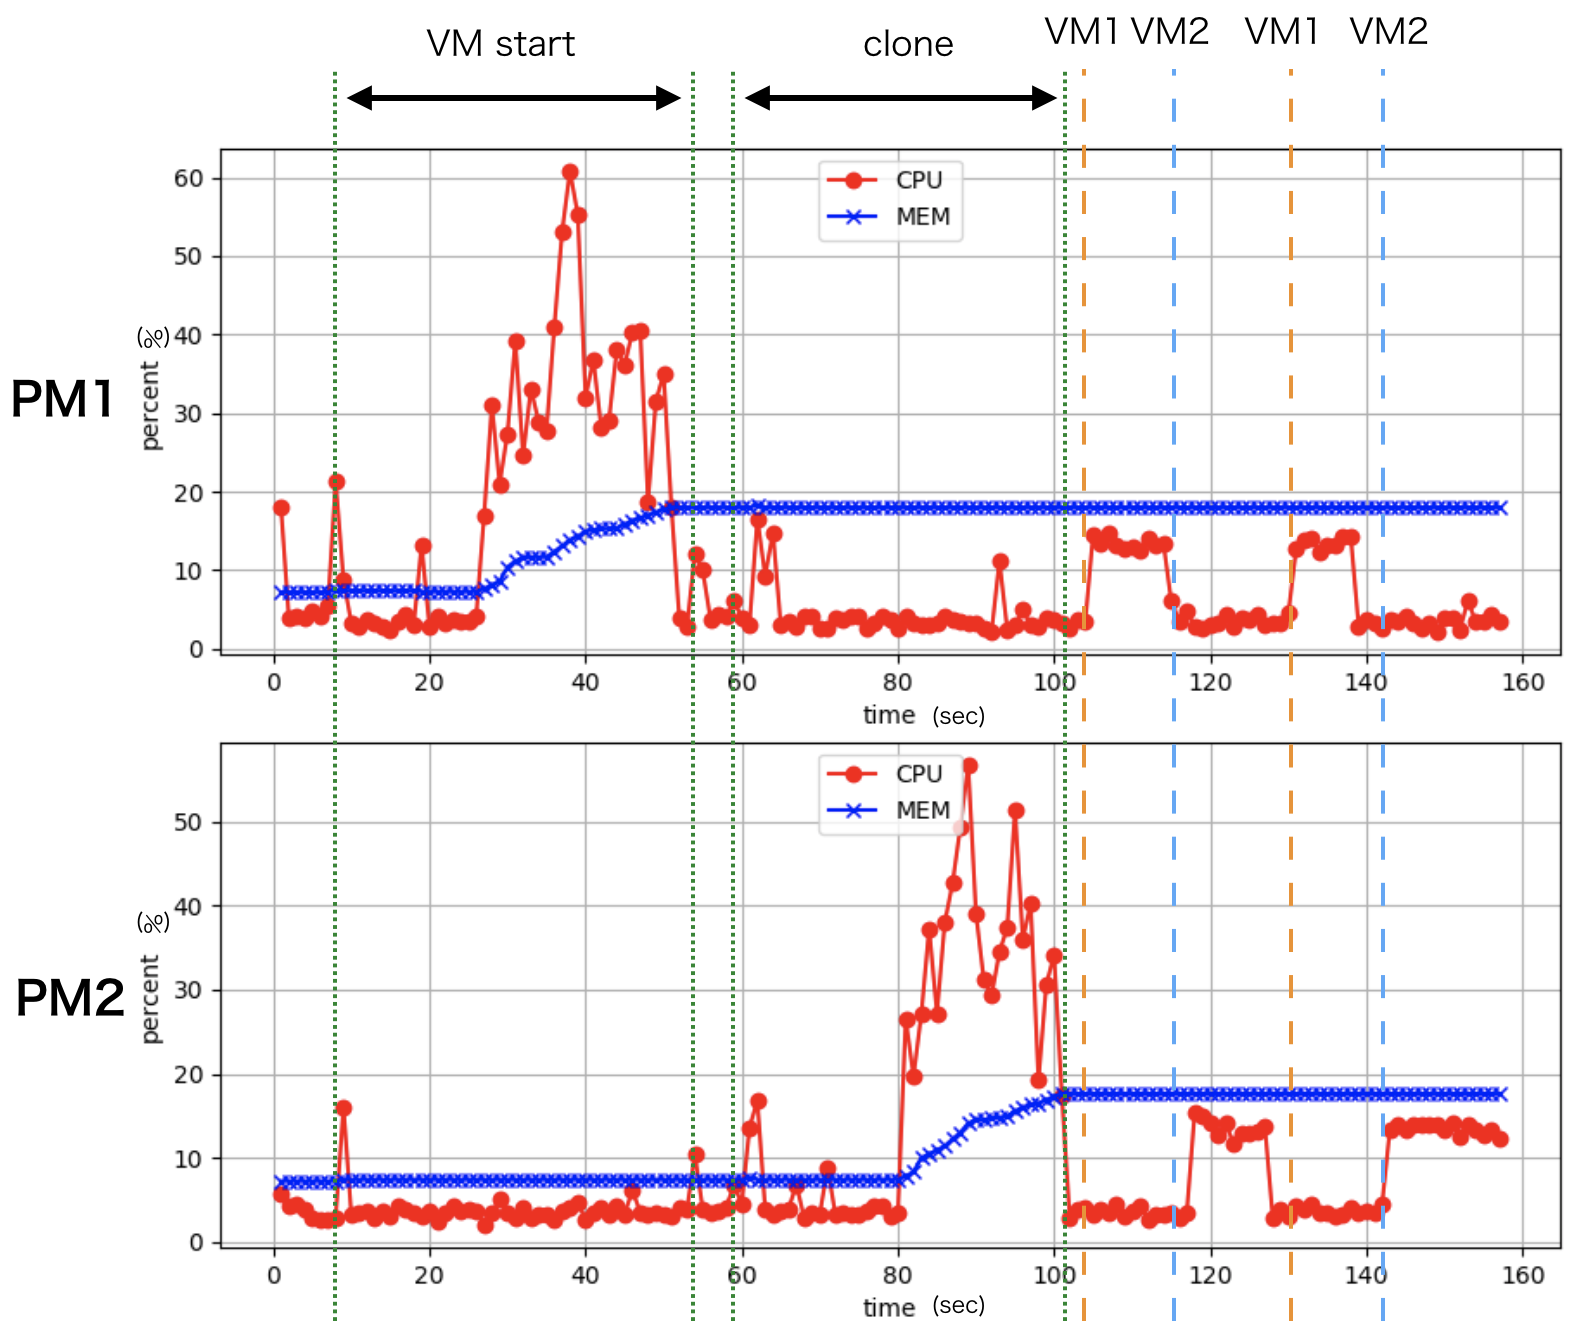
\includegraphics[width=9.0cm]{fig/clone.png}
	\caption{負荷分散によるリソース推移}
	\label{fig:graph_clone}
\end{figure}

次に仮想マシンの複製による負荷分散では,移動と同様に,PM1で仮想マシンが実行され,
約30秒かけて起動が完了する.その後,スナップショットを転送する時に,
CPU使用率が上昇する(図\ref{fig:graph_clone}, 65秒付近).スナップショットの
転送が完了すると,PM2で転送されたスナップショットを指定して仮想マシンの起動が
行われる.複製完了後,PM1へHTTPアクセスを開始する(図\ref{fig:graph_clone},
破線PM1).通常はクライアント毎にアクセスを分散させるが,今回はリソースの変化を
見るために,25秒ごとにアクセスを分散させた.PM1にアクセスが届いている間,
PM1ではCPU使用率が10\%程度上昇し,PM2ではリソースに変化がなかった.
次に,リクエストがPM2へ転送が行われるようにネットワーク構成の変更を行うと,
(図\ref{fig:graph_clone},破線PM2),PM1ではCPU使用率が下がり,
PM2ではCPU使用率が10\%程度上昇した.その後もPM1へ転送が行われるように
ネットワーク構成の変更を行うと,PM2ではCPU使用率が下がり,PM1では
CPU使用率が10\%程度上昇した.この振る舞いは表\ref{tab:func_time}の結果と
ほぼ一致しているため,リソース使用率の変化を正しく計測できていると考えることが
できる.また,負荷の分散が行われていることが確認できたので,本機能が想定通りに動作していると言える.

\begin{figure}[t]
	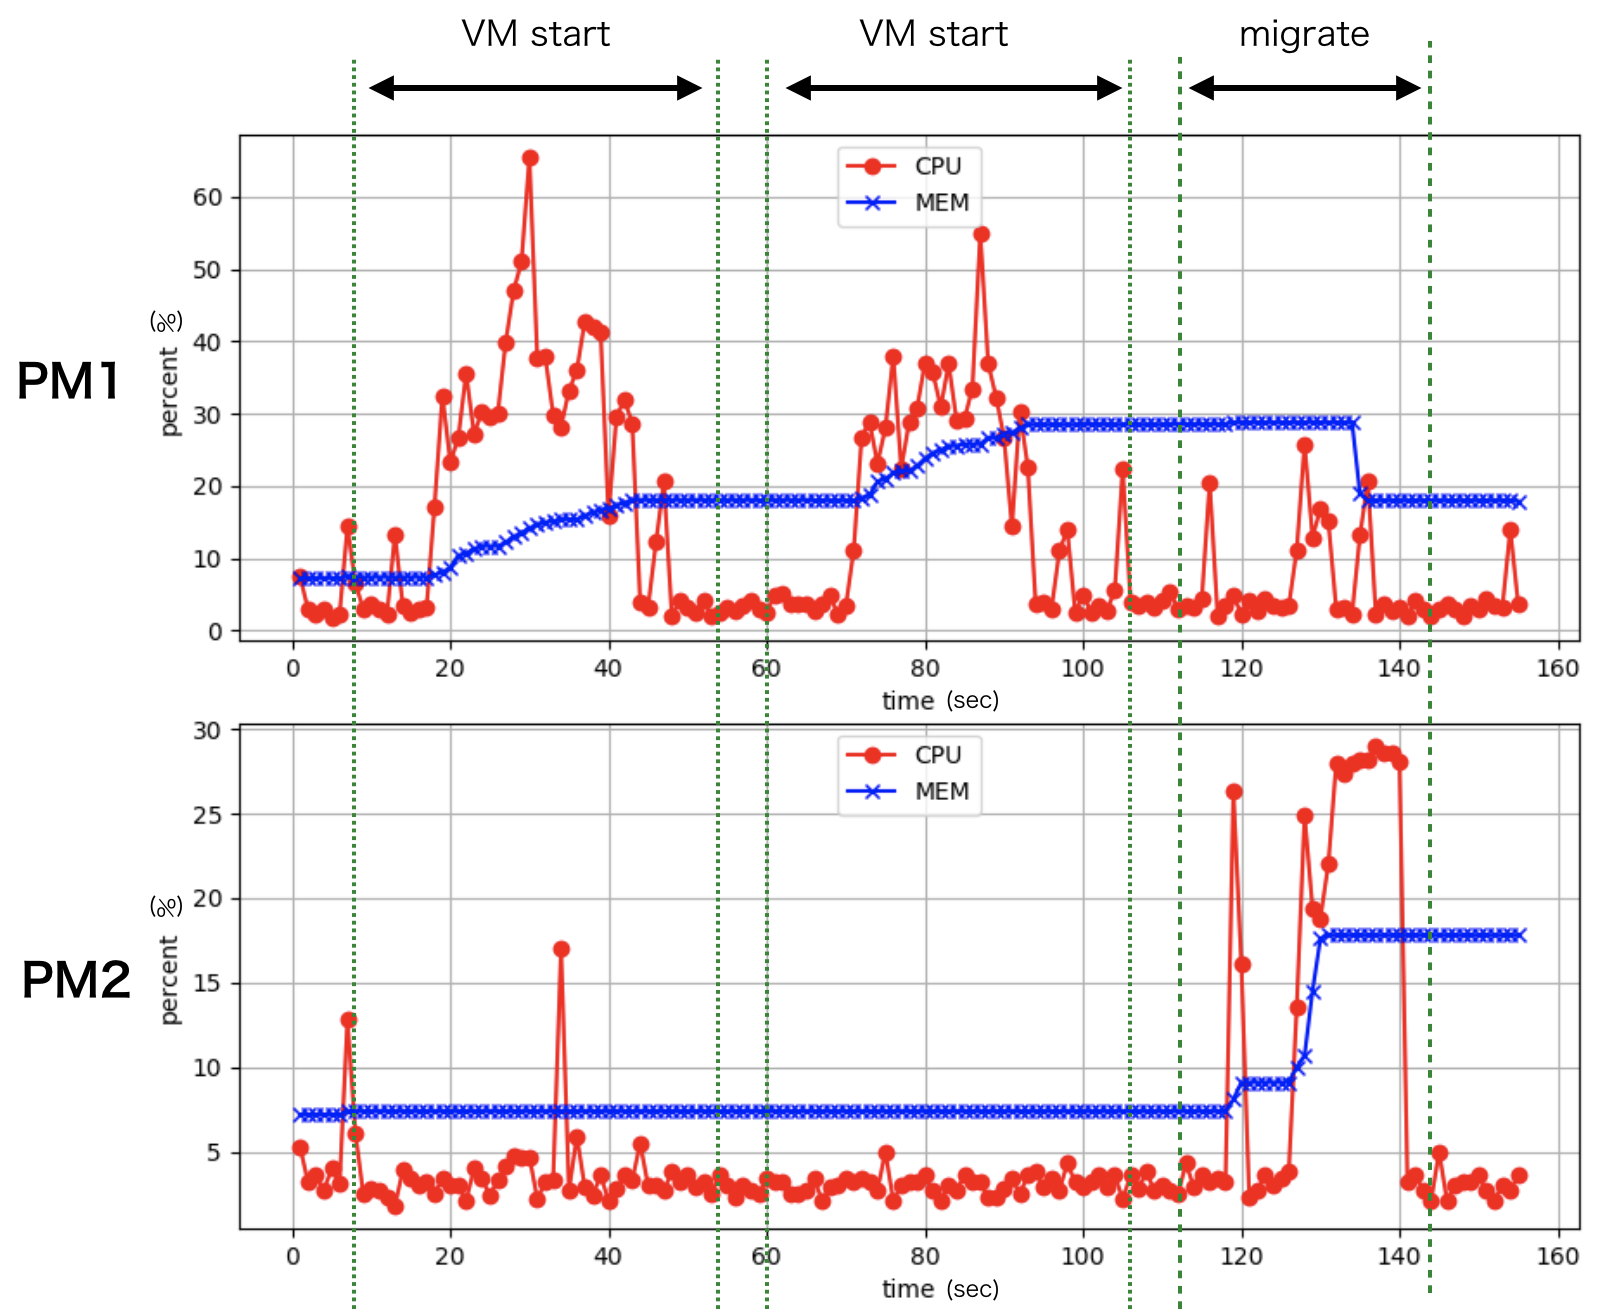
\includegraphics[width=9.0cm]{fig/migrate_vm2.png}
	\caption{仮想マシンを複数起動した状態でのリソース推移:移動}
	\label{fig:graph_migrate_vm2}
\end{figure}
\begin{figure}[t]
	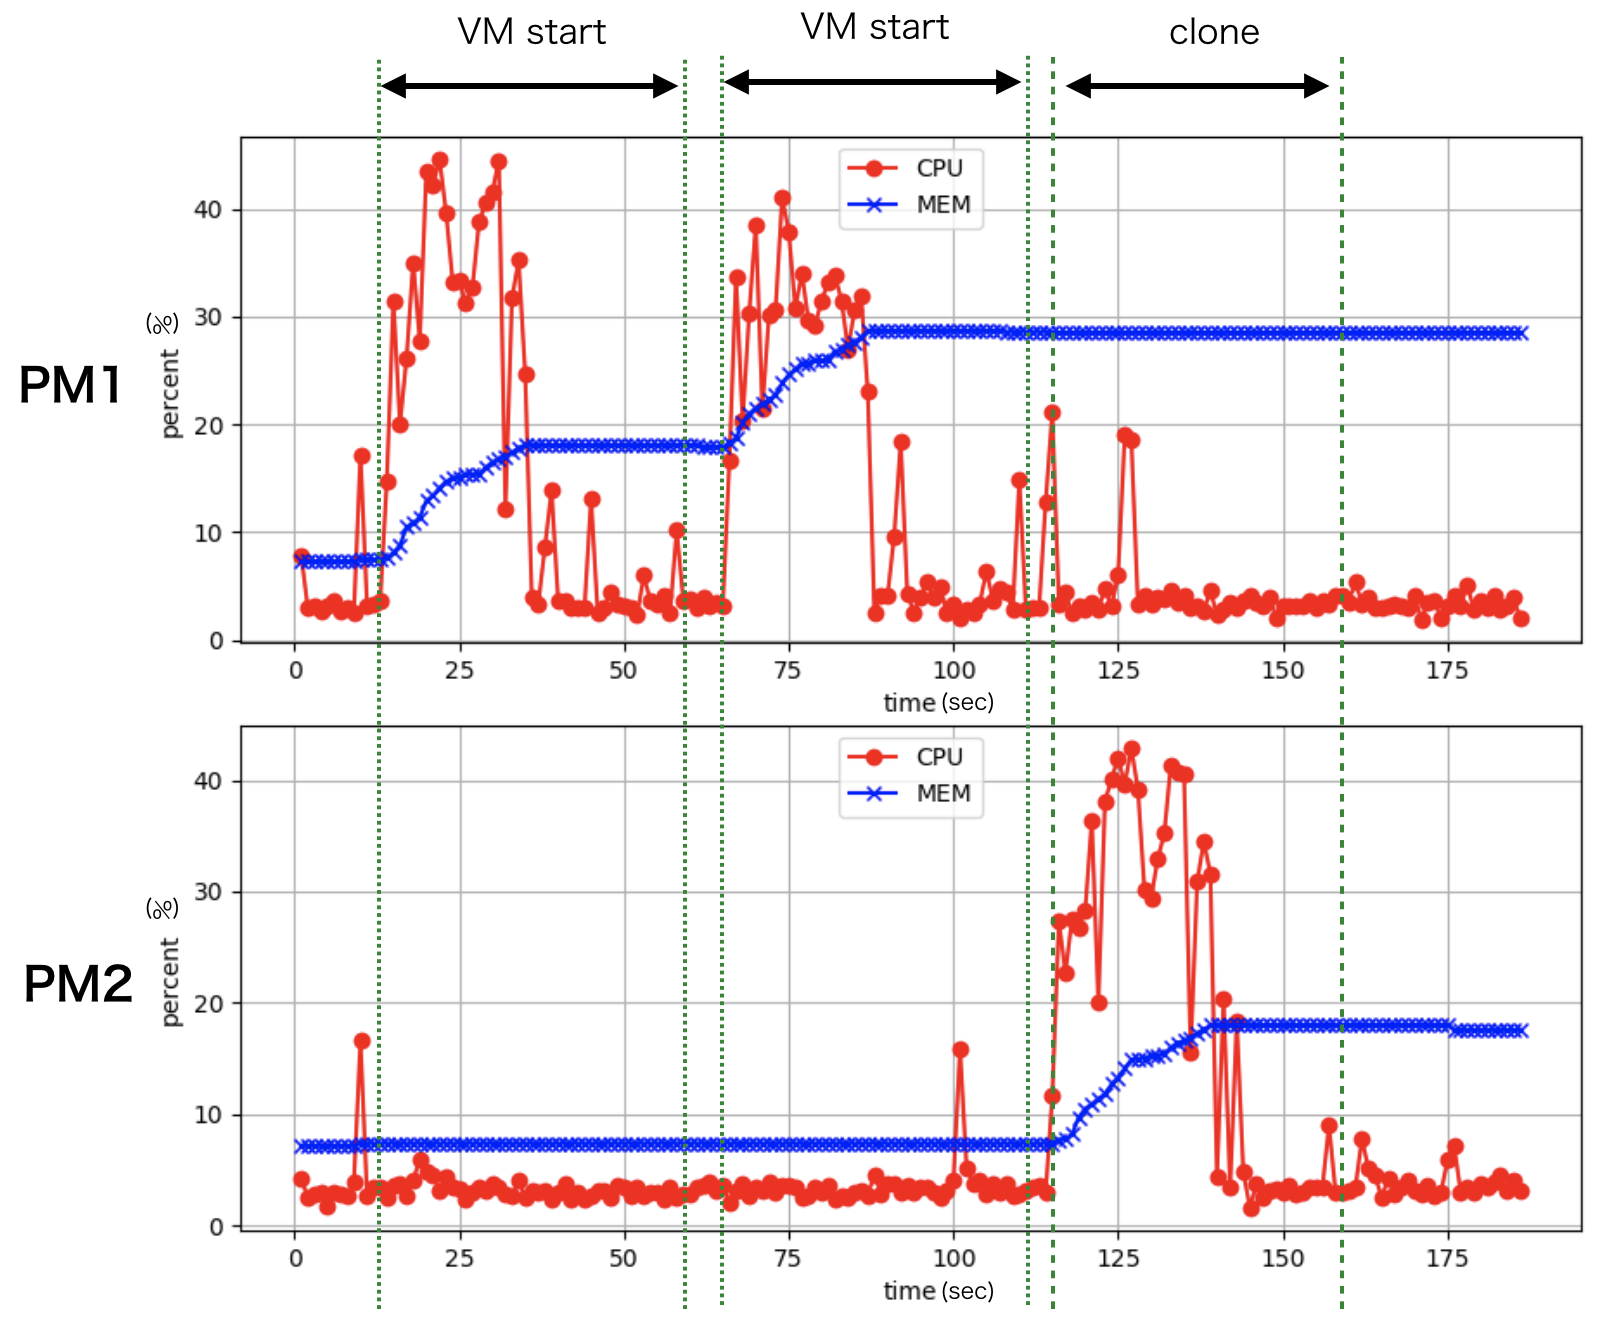
\includegraphics[width=9.0cm]{fig/clone_vm2.png}
	\caption{仮想マシンを複数起動した状態でのリソース推移:複製}
	\label{fig:graph_clone_vm2}
\end{figure}

最後に一台の物理マシンで仮想マシンを複数起動した状態において,一台の仮
想マシンの移動と複製を行なった場合のリソース使用率の変化を図
\ref{fig:graph_migrate_vm2}, \ref{fig:graph_clone_vm2}にそれぞれ示す.
これまでの結果同様,仮想マシンの実行が開始されるとCPU,メモリ使用率が
増加し,起動が完了するとCPU使用率は実行前と同等の値となる.一方,メモ
リ使用率は起動している仮想マシンの個数に応じて増加している(一台あたり
約10\%使用).そして.仮想マシンの移動や複製が行われると,移動した仮想
マシンの個数に応じて移動先物理マシン(PM2)のメモリ使用率は増加し,反対
に移動元物理マシン(PM1)のメモリ使用率は減少する.

これらのことから,一台の物理マシンで複数の仮想マシンが実行される場合で
も,本テスト環境では正しくリソース使用率を計測していると考えることがで
きる.

\begin{figure}[t]
	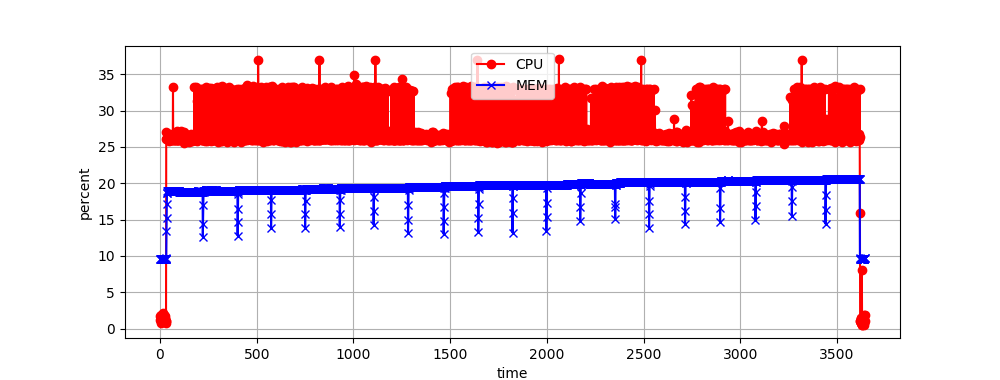
\includegraphics[width=9.0cm]{fig/kawaii.png}
	\caption{分類器の作成を行なった時のリソース推移}
	\label{fig:kawaii}
\end{figure}

\subsection{分類器の作成}
最後に,RaspberryPiで分類器の作成を行なった時のリソース推移を図\ref{fig:kawaii}に示す.
分類器の作成はOpenCV2\cite{opencv2}のカスケード分類器\cite{cascade}の作成を行なった.
今回は正解データ60枚,不正解データ30枚で実験を行なった.
その結果,CPU使用率は25~35\%,メモリ使用率は20\%使用された.
このことから,1台のRaspberryPiで2つの分類器の作成を行えることがわかった.
しかし,図\ref{fig:kawaii}に示すように,1時間の時間を要した.
これは,分類器の作成を行なってから1時間後にその結果が反映されることになるので,RPCとしては機能していないことがわかる.
CPU,メモリの使用率が100\%になっていないことから,単純にRaspberryPiの性能によるものだと推測される.

\section{まとめ}
本研究では,ロボットの探索能力とディープラーニングの判別能力を活かしかわいいものを探索するシステムを開発した.
これにより,対象物の情報を収集することに成功した.
しかし,本稿で説明したRPCシステムは本研究で成果を残すことができなかったため,今後より効率的なシステムの運営が行えるように改良する必要があることがわかった.

\subsection{今後の課題}
今後の課題として,分類器の作成に時間がかかってしまう問題は,分類器の作成を分散処理させ,高速で分類器の作成を行うように修正する必要がある.
また,対象物を拡張し,様々な情報収集を行えるようにするなどが挙げられる.

%%%%%%%%%%%%%%%%%%%%%%%%%%%%%%%%%%%%%%%%
%%参考文献
%%%%%%%%%%%%%%%%%%%%%%%%%%%%%%%%%%%%%%%%
\begin{thebibliography}{10}

% \bibitem{kawaii1}
%   大倉典子,青砥哲朗 "かわいい人工物の系統的研究" 第2回横幹連合コンファレンス, 2007

\bibitem{thesis2}
M.Ohkura, and T. Aoto : Systematic Study for “Kawaii” Products, Proceedings of the 1stInternational Conference on Kansei E;lngineering and Emotion Research 2007 Sapporo, Oct. 2007.

\bibitem{thesis3}
  大倉典子,後藤さやか,村井秀聡,青砥哲朗:バーチャルオブジェクトを利用した「かわいい」色の検討、日本感性工学会論文誌, vol.8,no.3,pp.535-542, May, 2009.

  \bibitem{roomba}
    ロボット掃除機 ルンバ|アイロボット公式サイト-iRobot https://www.irobot-jp.com/roomba/ 2017/07/24

\bibitem{kinect}
  Xbox\ One用\ Kinect|Xbox http://www.xbox.com/ja-JP/xbox-one/accessories/kinect 2017/07/24

\bibitem{ros}
  Ros Wiki http://wiki.ros.org/ 2017/07/24

\bibitem{rpi}
  Raspberry Pi - Teach, Learn, and Make with Raspberry Pi https://www.raspberrypi.org/ 2017/07/24

  \bibitem{raspbian}
    Raspbian\ Jessie\ Lite https://www.raspberrypi.org/downloads/raspbian/ 2017/07/14

  \bibitem{thesis1}
    Fung Po Tso, David R. White, Simon Jouet, Jeremy Singer, Dimitrios P. Pezaros School of Computing Science, University of Glasgow, G12 8QQ UK, "The Glasgow Raspberry Pi Cloud: A Scale Model for Cloud Computing Infrastructures", 2013 IEEE 33rd International Conference on Distributed Computing Systems Workshops

\bibitem{aws}
   Amazon Web Services website. https://aws.amazon.com/jp/ 2017/04/19

\bibitem{azure}
    Azure website. https://azure.microsoft.com/ja-jp/ 2017/07/14

    \bibitem{virt}
      virt-manager website. https://virt-manager.org/ 2017/04/19

    \bibitem{qemu}
      qemu website. http://www.qemu.org/ 2017/07/14

    \bibitem{sdn}
      Open Networking Foundation website. https://www.opennetworking.org/ 2017/01/11

    \bibitem{opf}
      Open Networking Foundation OpenFlow website. https://www.opennetworking.org/sdn-resources/openflow 2017-01-11

      \bibitem{iperf}
        iperf website.  https://iperf.fr/ 2017/04/19

\bibitem{snapshot}
   http://wiki.qemu.org/Documentation/CreateSnapshot 2017/07/20

\bibitem{opencv2}
  OpenCV2 http://opencv.jp/ 2017/07/25

\bibitem{cascade}
  カスケード型分類器 — opencv 2.2 (r4295) documentation - OpenCV.jp http://opencv.jp/opencv-2.2/c/objdetect\_cascade\_classification.html  2017/07/25

\end{thebibliography}
\end{document}
